\documentclass[paper=a4, fontsize=12pt]{main}
\usepackage{graphicx}
\usepackage{hyperref}
\usepackage{listings}
\usepackage{amsmath}
\usepackage{array}
\usepackage{enumitem}
\usepackage{xcolor}
\usepackage{setspace}
\doublespacing
%%%%%%%%%%%%%%%%%%%%%%


\definecolor{codegreen}{rgb}{0,0.6,0}
\definecolor{codegray}{rgb}{0.5,0.5,0.5}
\definecolor{codepurple}{rgb}{0.58,0,0.82}
\definecolor{backcolour}{rgb}{0.95,0.95,0.92}

\lstdefinestyle{mystyle}{
    backgroundcolor=\color{backcolour},
    commentstyle=\color{codegreen},
    keywordstyle=\color{magenta},
    numberstyle=\tiny\color{codegray},
    stringstyle=\color{codepurple},
    basicstyle=\ttfamily\footnotesize,
    breakatwhitespace=false,
    breaklines=true,
    captionpos=b,
    keepspaces=true,
    numbers=left,
    numbersep=5pt,
    showspaces=false,
    showstringspaces=false,
    showtabs=false,
    tabsize=2
}
\lstset{style=mystyle}

%%% Input project details
\newcommand{\studentname}{Octavio del Ser}
\newcommand{\reportyear}{2019}
\newcommand{\projecttitle}{ Architecture for application of learning methods for the reconstruction of action models.}
\newcommand{\supervisorname}{Prof. Sara Bernardini}
\newcommand{\degree}{Msc (Hons) in Computer Science}
\newcommand{\fullOrHalfUnit}{Full Unit} % indicate if you are doing the project as a Full Unit or Half Unit
\newcommand{\finalOrInterim}{Final Report} % indicate if this document is your Final Report or Interim Report
\begin{document}
\setcounter{tocdepth}{3}
\setcounter{secnumdepth}{3}
\maketitle
% https://docs.google.com/spreadsheets/d/1cLyskq9Byp1fQ53CoebMgVGKxIqFYxIIhuRzzX_gvXY/edit?usp=sharing
%%%%%%%%%%%%%%%%%%%%%%
%%% Declaration

\chapter*{Declaration}

This report has been prepared on the basis of my own work. Where other published and unpublished source materials have been used, these have been acknowledged.

\vskip3em

Word Count:

\vskip3em

Student Name: \studentname

\vskip3em

Date of Submission: 23 April 2020

\vskip3em

% Signature: 
\newpage
%%%%%%%%%%%%%%%%%%%%%%
%%% Table of Contents
\tableofcontents\pdfbookmark[0]{Table of Contents}{toc}
All code is available on: \url{https://github.com/Occy88/AIPrinciples/tree/main/Planning/project}.
A diagram of all systems can be found in the root of the Github. I advise against attempting attempting to run this as it is intensive, and requires replacement of some pip packages with patched ones.

\newpage

\begin{abstract}
%what am I writing about and what is it's usefullnes/point of it.

Automated planning has been a topic of research since the 1960s. It came into fruition due to the desirability of accomplishing tasks autonomously, which is a problem in almost all activity-based domains. Tasks are solved by an ordered set of actions over a domain. The job of formally defining actions, their conditions and effects, becomes increasingly difficult and prone to error as domains evolve to be ever more complex. For such reasons, in recent years, researchers have leveraged progress in Machine and Deep learning to automate the generation of action models from synthetic and real-world data. Machine learning a deep learning techniques are evolving at an increasingly fast rate, whilst there has been no clear translation layer between action models and common learning libraries. Combined with the multitude of existing domain languages, This issue has manifested itself as lack of testing and use-able implementations of current reconstruction approaches.

% Summary of what was done in this Disertation
This dissertations provides an overview of the current state of the art in reconstruction of action models, discusses core issues that have affected rapid development and implementation of more powerful reconstruction techniques available today, and proposes a framework standardising future development of  action-model reconstruction models. A proof of concept framework is then tested with an existing learning model using Markov Logic Networks, finally we compare results. 

% Summary of results/observations.
We have found that the proposed framework can work in the simulated scenario and provides a good foundation for more complex learning model implementations. Being based in python is highly modular and provides possible integration with all modern learning techniques. This framework also lowers the entry barrier for new researchers in the field as there is no longer a need to question language format or how to implement it as most existing languages can be supported over time.



% quick intro


% what I'm doing

% what i've done\newline
% software eng


% challenges I've faced

% challenges/next term

\end{abstract}

\chapter{Introduction}

\cite{ReviewActionModels:article}

% what is the problem space
% Some examples
% How do the above examples tie in with issues faced
% What needs to1 be answered in order to create the system that we propose (rethorical)
% Which of these has been attempted how did it work out, -> hence us doing it.

% What is automated planning/ reconstruction
This dissertation focuses on Automated Planning (AP), a well-established branch of artificial intelligence that
concerns itself with the generation of strategies or plans typically fulfilled by intelligent agents such as
(Warehouse robots, Assembly line robots, UAV's, MAV's, home roomba type robots).

A plan or plan trace is defined by a series of actions meant for the execution on an initial state space
transitioning it to a pre-defined goal state. Executing such a plan accomplishes a task such as the evasion
of an obstacle or acquisition of an object.
%languages
The laws governing a state space (action-models, objects, relations) are usually interpreted by a formal language.
Many such languages exist today (PDDL, PPDDL, STRIPS, OCL, ADL), each created to improve expressiveness, ease of use,
or add desired functionality.
Such languages were introduced as an attempt to standardize the process of defining a domain and solving planning problems.
Languages are similar in their structure, a domain and a problem must be defined, which is then used by a compatible
solver to find a solution for the problem in said domain.

Knowledge Engineering (KE) for AP is the process that deals with the overall generation of domain models from existing
data (plans, actions, states), including the acquisition, formulation, validation and maintenance of knowledge for the
model \cite{AutomatedKETools:inproceedings}.

A common situation in KE is that the encoding of the domain left to a domain expert. Often being a laborious and complex task,
it makes future maintenance difficult whilst also being prone to human induced error, testing is also a non-trivial task.
This issue compounded with the ever increasing complexity of real-world scenarios thanks to advancements in computation
and commercial need for automation, means that the challenge of engineering domain models is ever-more challenging.
In an effort to tackle this issue and assisting domain experts in modeling domains, new systems are constantly
being researched and developed for the automatic acquisition of AP models.

Existing state of the art planning algorithms such as AMAN, LOPE, ARTUE, ARMS and more \cite{ReviewActionModels:article}
rely on a multitude of different learning based approaches, such as reinforcement learning, MAX-SAT,
supervised learning and transfer learning. Each of these algorithms also rely on specific input
data and output action models in different languages. This added complexity makes it difficult for anybody without
expertise in a particular implementation, of using newly developed techniques. It has also been observed that working
examples of implementations are difficult to obtain and test due to the lack of standard data generation techniques
often provided by online resources which no longer exist.

The variance in development standards and models produced in this field, demonstrates a clear lack of organization and
management of existing algorithms, techniques and development standards.
An argument could be made that a lack of commercial appropriation of such niche techniques
(in industry) made the development of libraries comparable to Tensorflow or Pytorch overly laborious and
time-wise uneconomical for individuals. However the lack of such robust and readily available code makes teaching and
implementation or even experimentation of existing techniques unnecessarily complex often causing 3rd parties to avoid
implementations by researchers. We also have to consider the constant evolution of programming languages.
As time goes on and problems become more complex, hence there is a constant shift towards more abstract/higher level languages.
This is thanks to their inherently improved legibility and development speed often at the cost of execution speed.
For such reasons most complex algorithms and data structures are usually written in lower level languages
such as C/C++ and then wrapped by most popular higher level languages for easy implementation such as GO and Python,
this has not been the case with Domain languages as language standards created tens of years ago are still in common use today.


As a result of issues discussed, we can observe that teaching bodies or inexperienced users often resort implementing
planning problems from scratch, using custom data structures and algorithmic implementations in higher level languages
such as python due to their comfort; rather than implementing a domain using a Domain language and a solver in
their preferred higher level language. This situation is fine for the individual case, hwever it also translates
to more advanced use cases as people grow used to the tools they are taught.

% What are the key objectives from the above (to solve/analyse/future improvement)
% What was the goal and where does it stand int he dissertation
% How are results evaluated (where in the disseratation/what was done) / any difficulties
% 
%Objectivesz
% Methods
% Results
% Conclusions
We ask ourselves, what needs to be done in order to tackle these issues.
The two most important tasks that we believe need to be tackled are as follows.
First is that a solution needs to be useful for researchers in the field,
mainly saving them time and effort when developing new ideas.
This means the solution needs to be highly adaptable/modular to any environment allowing for constant improvement and extension.
It also has to aid in mundane tasks such as data generation and management for testing and implementation.
This allows for more accessible and robust and verifiable implementations.
Examples exist for machine learning, such as importing of pre-processed datasets (mnist etc...) directly from a package.
Secondly the system needs to be simple and robust for users alien to the field.
This requires good documentation, and high level access to existing algorithms without the need to open the guts of a particular implementation.


Given the above we propose a framework with an initial proof of concept built in python,
integrating a custom implementation of a single algorithm for reconstruction of action-models using Markov Logic Networks,
and test this implementation against existing data.
Our objectives for the framework are as follows:
% Todo: review
\begin{enumerate}
    \item Support for parsing various domain languages to a python standard.
    \item Synthetic generation of training data.
    \item Simplified implementation of learning models.
    \item Extendable modules for conversion of training output to a standard action model.
    \item Testing framework for learned action models.
\end{enumerate}

\chapter{Background and Theory}
In this chapter, we discuss the theory underlying the core issues we are trying to tackle. We outline the concepts that make up the current state of Automated Planning, such as domains, languages, solvers and more. We then explore examples tools, learning models and solvers that have been developed to date, such as pracmln a python based Markov Logic Network learning tool, AMAN an uncertainty based approach for learning action models, ARMS a MAX-SAT based approach for learning action models, PDDL a domain language and ffx a solver. We will use the theory to draw conclusions relating to the feasibility and requirements to achieve the goals outlined in the introduction for this project.


\section{Modelling Domains}
Creating a complex system in which agents act independently of user input can be a highly complex task. An agent within such a system must generate a plan in order to define which actions are optimal given the state of the environment (Domain) in which it exists. A planner may often require knowledge of other agents within the domain in order to distribute work more effectively, for this reason a language providing the ability to model such a domain is required. Such a language also allows existing planners to solve for defined problems without knowledge of the domain. Many languages exist the most prominent of which is STRIPS. \newline
STRIPS was the name given to a component in charge of planning for the software used in Shakey the robot developed by the Stanford Research Institute. Shakey was the first machine to be able to reason about it's own actions there for a sort of ancestor to modern autonomous agents. Shakey had multiple relatively basic abilities (visual analysis, object manipulation and more), what made Shakey impressive was the ability to received a set of goals to achieve and using the STRIPS planner generate the required actions to get as close to the desired solution.
\newpage
\subsection{STRIPS}
An instance of STRIPS (Stanford Research Institute Problem Solver) can be represented as a quadruple \(\{P,O,I,G\}\)
\begin{itemize}
  \item \(P\) is a set of propositional variables (represents a given state)
  \item \(O\) is a set of operators (actions) each of which is in itself a quadruple \(p_{true},p_{false},p_{add},p_{del}\), each item representing a set of propositional variable required as a precondition (true/false) or as an effect (add/del) of an operator.
  \item \(I\) is the initial state, just like \(P\) it is a set of propositional values that are initially true.
  \item \(G\) is the goal state represented as a tuple \(\{g_{true},g_{false}\}\), each a set of propositional values that must be True or False in  order for the goal to be deemed as achieved.
\end{itemize}
A plan for a given STRIPS instance is a sequence of operators that upon execution from the initial state leads to the goal state.

\subsection{PDDL}
PDDL  (Planning Domain Definition Language) is a framework designed to standardise domain, problem and planning languages. As previously discussed, STRIPS is not the only language. PDDL was created in order to make the yearly International Planning Competition (IPC) possible. This competition evaluates the performance of proposed planning systems on a set of well known bench-marked problems, hence a standardised language for defining such problems was required. Many planners do not support the full extent of PDDL, and instead focus on the most popular requirements listed in the PDDL specification, these include (STRIPS, ADL, typing, existential preconditions,equality, conditional effects ) and more. PDDL has evolved over the years and new ever more complex releases were created in order to support the ever increasing complexity of planning tasks. PDDL 2.1 adds durative actions and inequalities and PDDL 3.0 adds prefrences and contstraints. 

An important note about planners is that they not only do not support full PDDL, but depending on the planner, there may only work correctly on a specific format. These formats can be things such as requiring action preconditions/effects to be written only as conjunctions. most planners may ignore the "requirements secion of PDDL", hence when testing a planner on a problem, one cannot assume it will work unless tested or documentation is provided.

One of the largest most up to date websites for identifying PDDL requirements and active usage is the planning.wiki website where up to date documnetation of the PDDL standard is provided.

PDDL consists of a domain file and a problem file. The PDDL domain file consists of a set domain definition types (such as actions, durative-actions, functions, axioms, requirments, types.) defined by the PDDL version in use. the PDDL Domain defines the "rules" of the world upon which a problem is defined. The problem file is made up of four components. A reference to a domain upon which the problem is based

\section{Parsers}
Parsing is important because it allows us to translate a language into another. In our case we want to simulate a PDDL Domain in python, hence we require a parser to interpret PDDL and convert it to a relevant data structure. We want to make our framework as open, modular and easy to use as possible, hence we need to be able to convert different domain languages into one python based simulator, and considering that languages evolve, so must the translation layer. Parsers are perfect for this job because they convert a formal language with specific rules using Lexical Analysis into Tokens, constructing a tree which can then be translated into a new language. Parsers are considered to be mature, most modern programming languages provide very comprehensive parsing toolkits allowing for the efficient interpretation of a language, especially if it's grammar is well defined.
% Solvers & outputs
\begin{figure}[h]
\centering
 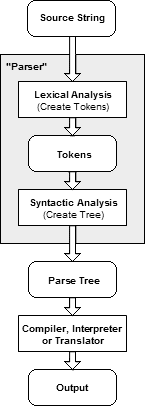
\includegraphics[height=300px]{images/parserflow}
 \caption{Parsing process architecture.}
 \label{fig:parserflow}
\end{figure}
\ref{fig:parserflow} represents a common case of a parsing flow, in this case parsing a computer language \cite{ParsingW23:online}. The first stage of the parsing process involves converting an input stream of characters into tokens (set of characters) defined by a grammar (regular expressions) written for the language being analysed. A lexer ensures that the generated tokens are meaningful by leveraging grammar defined for the language. Once tokens are generated the next stage is syntactic analysis in order to check that tokens are in the correct order and format. Grammar definitions are usually written with context-free format, which defines layers of components that can appear in the language in a recursive manner, for example, a top level component such as a book will be composed chapters, paragraphs and sentences. Syntactic analysis usually generates a tree that is then ready for parsing and interpretation. This section is what allows us to convert data in a previously cumbersome format such as text into a useful format such as a custom data structure in a given language.

Given the above specification, we can observe that writing a parser from scratch is cumbersome. For this reason most common languages today offer parsing toolkits which allow for efficient construction of parsers by taking care of the heavy lifting, meaning a developer only has to defined a grammar file for the parser to construct a tree from and a transformer to convert the tree into a desired format. Existing toolkits include ANTLR, Lark, JavaCC, SYNTAX and more, each with their advantages and disadvantages. When choosing a toolkit, we must account for cross compatibility between languages, speed, memory usage, supported features.
\newpage
\section{Solvers}

Solvers for a classical planning problem usually center around the same three requirements. A characterization of an initial state, a set of goals and a set of possible actions. Solvers are then expected to synthesize a sequence of actions that when executed in the initial state will transition the world to satisfy the goal state.

A classical planning problem is based on the following assumptions:
\begin{enumerate}
\item  The state space of the planning task is finite and fully observable.
\item Actions are deterministic and instantaneous.
\item Goal attainment is complete (not partial).
\end{enumerate}

Existing solvers are language specific, meaning that they support a specific domain language and venturing outside of this specification will break the functionality of the solver. This is important because as languages and problems evolve so must the solvers, meaning that a robust system must account for solver compatibility. As an example we can take the well known Fast Downward solver published in 2004 \cite{FastDown46:online}, since then there have been upwards of 6 iterations over the initial implementation, the most recent in 2018. 
% TODO: Solver Diagram flow.



\section{Markov Logic Networks}
As we will be implementing an action model reconstruction algorithm to demonstrate the effectiveness of development with our framework, we chose to use Markov Logic Networks for our learning model. A python package called pracmln \cite{pracmln} developed for the specific purpose of learning action models using Markov Logic Networks. This section describes the theory, advantages and disadvantages of MLN's.

The purpose of Markov Logic Networks was to efficiently handle uncertainty or noise in data by combining probability and first-order logic. Traditional first-order logic permits a compact representation of predicates forming Knowledge Bases. Probabilistic graphical models such as Bayesian Networks allow for the efficient handling of uncertainty and provide flexible and efficient querying of probabilities. Today's practical applications require both the KB's and probabilistic models to tackle situations where uncertainty such as noise is a factor. MLN's combine both probability and first-order logic, with the only restriction being that the domain must be finite. Algorithms exist for learning (or training) and inference of such networks. 

A Markov logic network consists of a first-order knowledge base where each formula has a weight attached to it. These networks can be interpreted as "simple" templates for constructing large Markov Networks while incorporating rich domain knowledge.

\subsection{Markov Networks}
Markov networks fall under the branch of Undirected Graphical Models. 
They are represented as a set of random variables forming an undirected graph that must satisfy Markov properties. Markov Networks are often compared to Bayesian Networks, however there are some key differences. Unlike Bayesian Networks, which are acyclic and directed, Markov Networks can be cyclic and are undirected. Therefore there are dependencies that Markov Networks can represent (e.g., cyclic) that Bayesian Networks cannot and vice versa (e.g., induced).
Each maximal clique in the graph has a corresponding real-valued non-negative function (so-called potential function). The values of these potential functions can be viewed as how well-correlated nodes are within the clique.

Given an undirected graph \(G = (V,E)\) , V being vertices, E being edges.
A set of random variables \(X = (X_v)_{v\in V}\) form a Markov random field with respect to \(G\) if they satisfy the following three Markov properties \cite{Markovra75:online}:
\begin{enumerate}
\item Pairwise Markov property: Conditional independence of any two non-adjacent variables given all variables: \[X_u \perp\!\!\!\perp X_v \mid X_{V\setminus\{u,v\}}\]
\item Local Markov property: Conditional independence of a variable to all other variables given its neighbors: \[ X_v \perp \!\!\!\perp X_{V\setminus N[v]} \mid X_{N(v)}\] \(N(v)\)  is the set of neighbors of \(v\). \newline\(N[v] = v\cup N(v)\) representing the closed neighbourhood of \(v\).
\item Global Markov property: Conditional independence of any two subsets given a separating subset.
\[X_A \perp \!\!\!\perp X_B \mid X_S \]Separating subset meaning that any path linking nodes from \(X_A\) to \(X_B\) must pass through \(X_S\) the separating subset.
\end{enumerate}

In Bayesian Networks, the chain rule is used to build joint distributions from conditional probability distributions. Hence the use of conditional probability tables (CPD's) in order to facilitate computation of a specific query on the graph. In the case of Markov Networks we wish to calculate the potential value between two connected nodes. This is a real number as opposed to a probability between 1 and 0 as in Bayesian Networks. For Markov Networks a factor is assigned for each maximal clique which is then used to determine the probabilities of variables given a Network state.
To calculate the joint distribution of a Markov Network, the following formula is used: \[P(X=x) = \frac{1}{Z}\prod_k \phi_k(x_{\{k\}})\]
\(x_k\) is the state of variables appearing in the \(k^{th}\) clique.
\(Z\) the partition function defined as \(Z=\sum_{x\in X}\prod_k \phi\_k(x_{\{k\}})\)
\cite{mlj05pdf51:online}
\subsection{First-Order Logic (KB)}
A first-order logic knowledge base is a set of formulas written in first order logic which represent facts (hard constraints) on a set of possible worlds. Any world violating any of the constraints would be considered as having 0 probability of existence. 

Sentences in a first-order KB are constructed using four types: functions, predicates, variables and constants. Functions return a variable or a boolean e.g. divides(x,3) would return true if x is a multiple of 3. Predicates are a combination of two terms forming a relationship e.g. red house. Variables are variables as in any programming languages, they are a  placeholder for anything in a domain e.g. x representing numbers as seen in the Functions definition or the function itself. Constants are what what variables would hold at any given point during an operation, this can be any form of data such as a number or a string e.g. 1, house_1, 2 . 

First-order logic KB's allow us to do inference. The most common common representation is in the form of Horn clauses (contain at most one positive literal) this allows programming languages such a Prolog to search for statements taht hold in the KB.

\subsection{Markov Logic Networks}
The basis of MLN's is to build on first-order KB's by softening the effect of a constraint of the viability of a given world. Instead of stating a world is impossible if a constraint is not satisfied, we simply lower the likely-hood of the world by reducing the value of said constraint. Hence each formula in a MLN KB has a weight reflecting the strength of the constraint. The greater the weight of a constraint the greater the difference in log probability between a world that satisfies said constraint and one that does not (everything else remaining equal). 
\newpage
\section{Evaluating Models}
So far we have explored relevant theory behind all of the basic building blocks that will be used in the formulation of our framework except for the techniques used for evaluating action models, which will be an output of training. Evaluation of a learned model can be implementation specific, such as evaluating for performance under different but relevant conditions such as noisy, real or simulated environments. However we will go over the standard evaluation metrics for a learned model that apply most if not all modern ML situations. Before even training a model a the data used for training is split into training, testing and validation subsets typically in the 60/20/20 percentage range in order enable evaluation in later stages. Using these subsets of data, many evaluation metrics can be derived depending on the type of model being trained. In the general case for our framework we can say that our model falls under the classification type. We are creating a model that predicts an action which is not a quantitative value. For classification type models, the main metrics for evaluation are accuracy, precision and recall. As with all models, we must also look at the bias/variance trade-off metrics to ensure proper fit.

Accuracy is defined by the percentage of correct predictions on the test dataset by the model. \[ \text{accuracy} = \frac{\text{correct predictions}}{\text{all predictions}}\]

Precision is the probability that a prediction by the model is correct.
 \[ \text{precision} = \frac{\text{true positives}}{\text{false positives}+\text{true positives}}\]

Recall is calculated with respect to a class. It is the number of correct predictions for a class divided by the total number of elements that truly belong to the class.
\[ \text{recall} = \frac{\text{true positives}}{\text{true positives}+\text{false negatives}}\]

Accuracy alone is not good enough for evaluating the usefulness of prediction models as many cases exist where we are interested in predicting a class which represents a small subset of data such as disease. A model can be 90\%+ accurate by simply predicting nobody has said disease however it is useless when trying to identify people who are ill. For this reason, precision and recall provide the relevant metrics to identify the usefulness of a model. Commonly these two metrics are combined to for the f-score.
\[F_{b}=(1+b^2)\frac{\text{precision}*\text{recall}}{b^2*\text{precision}+\text{recall}}\]

\(b\) is a variable used to control the precision/recall trade-off, \(b\)<1 places more weight on precision whilst if it is greater than one recall becomes more important. When we want to ensure that all potential true samples are predicted, it is best to have a \(b\) > 1 as we want to maximize recall, precision can then be improved by subsequent analysis perhaps performed by humans, such as recognising cancer in images, or identifying people susceptible to suicide.

A model is trained on sample data hence it must generalize the knowledge learnt to some degree in order to make predictions on new samples. When a model is being trained on sample data, it attempts to fit the data to some degree, if a mode fits the training data too well, we say there is a high degree of variance as it places too much weight on individual data points, this means the model has been over-fit. On the other hand if not enough weight is placed on data points then there is high bias and a model is under-fit, an example of under-fitting would be approximating an exponential with a straight line. 
\begin{figure}[h]
\centering
 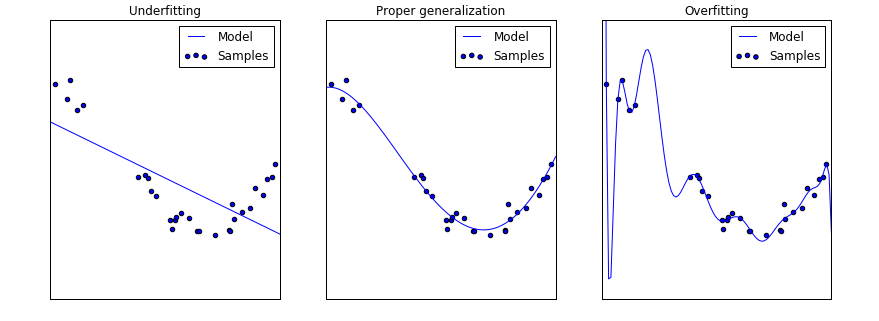
\includegraphics[width=\linewidth]{images/Selection_019}
 \caption{Bias vs Variance tradeoff.}
 \label{fig:bvtradeoff}
\end{figure}

Various tools exist for any framework when training a model in order to optimize this trade-off. A simple brute force approach involves performing a grid search by training a model multiple times with different hyper parameters. The hyper parameters that output the lowest mean square error would be the most optimal choice. Of course with more complex models and increasing number of hyper parameters, finding the optimal mean square error becomes more complex, which is why frameworks provide relevant tools for existing models. 

\newpage

\section{Existing work}\label{background:Existing Work}
We deem it important to review currently developed frameworks, learning models, and tools created by the community in order to ensure that we maximize what has already been developed by using what is available for our proof of concept implementation. there is no need to develop certain framework modules from scratch if we can tweak existing open source projects to our advantage and integrate them into our framework in order to demonstrate the flexibility and use-fullness of our design approach. 

We will review existing work associated with the five main targets outlined in our introduction in order to make sure that the work we review is closely associated with the problems we need to solve to make the framework a viable tool for development. 

\subsection{Support for various domain languages in python}
We discussed the reasons for providing support for domain languages in a higher level language, these including higher adoption rate by new developers, better legibility and compatibility with popular tools developed today. What is meant by support for a domain language in python, is essentially converting a language definition file into a well defined and tested python data structure. This data structure can then be manipulated and improved with ease as more languages are supported and tooling is improved.

Our main focus for this section is the conversion of PDDL to python. PDDL is one of the most popular planning languages today and python is the most popular programming language, which are the two most crucial factors influencing our choice. As python is so popular, multiple attempts have been conducted over the past few years to construct a PDDL parser based in python. We will provide a basic overview of the three most prominent open-source projects.

Pypddl-translator \cite{ssardina20:online} is a domain and problem PDDL parser written in python3 using PLY (Python Lex-Yacc) a parsing library. We decided to avoid this implementation due to a lack of testing, legibility and documentation. PDDL Supported functionality is defined, unfortunately errors were encountered when attempting to parse valid files due to poor coverage of PDDL requirements. PLY is also not a very popular parsing toolkit and is not as cross compatible with other languages as we would like to to be. For these reasons we have avoided inheriting from this project.

Pddl-lib \cite{hfoffani23:online} is a PDDL library that parses PDDL files using ANTLR4 grammar. It then exposes an API supporting Python 3.8. This API provides methods for obtaining the initial state, goals, operators, positive and negative preconditions as well as grounded states. This is the most sound implementation to date in python, however unfortunately it suffers of poor documentation and lack of testing. Few contributors have actively created pull requests for issues, however these have been ignored over several months. There is also no clear documentation of what has been implemented to date (supported version of PDDL and requirmenets). This makes continued development of the project difficult. Finally, the organization of resources is problematic as elements which should be separated are clumped into the same files, and contain no reference to the official PDDL paper \cite{httpsarx9:online}. Although the grammar used for parsing is popular and cross-compatible with many languages, the grammar file defined in the project lacks design definition, meaning without thorough investigation, it is very difficult to contribute to such a project without redesigning a large portion.

The last library we have reviewed is pddl-parser \cite{pucrsaut37:online}. This project conforms to modern development standards, ensuring builds are passing before merging new branches. Unfortunately  not parsing toolkit was used, instead files are parsed using python. Although for single use implementation this is ok, when a language expands or changes, these types of implementations often break as they assume a certain structure. Such an implementation is also difficult to test, modify and improve as code is much more illegible than standard parsing grammar.
Syntactic analysis is also done on the fly rather than from a tree which means any changes to the data structure that we wish to convert the parse tree to is borderline impossible. Finally such an implementation blockades use of the parser with python alone whilst most Parsing grammars offer integration with almost all modern languages.

In conclusion there is unfortunately no serious project currently being developed for parsing PDDL files, most implementation currently used in research and industry are custom and integrated directly with popular solvers making it difficult to integrate with. Hence the decision has been made to develop a formal parser for the PDDL 2.1 definition language. Design and initial implementation will be discussed further chapters.  

\subsection{Synthetic generation of training data}
Over the years many standard problems have been modeled in the planning community. Problems are usually catered to a specific level of complexity in order to allow researchers to accurately evaluate and compare new methods to existing ones. The most prominent issuer of such problems has been the IPC (International Planning Competition) which has been running since 1998 when Drew McDermott and a committee first created PDDL along with a collection of problems which defined the first benchmarks. Since then, every two years the series continued to progress with ever more difficult problems. These problems are released with a domain definition file and a generator which creates any number of goal states provided some hyper parameters. Planners are then bench-marked by their speed and ability to find optimal solutions for these problems. Well known problems include Blocksworld, Briefcaseworld, Gripper and Grid. 

What we have observed is that there is no lack of problems and generators for the acquisition of synthetic data, however it cannot be said that the process of doing so is straight forward. The most prevailing issues observed include lack of specification for execution of generators, meaning a user must find the correct compiler usually a version of C or C++ before usage. Common lack of documentation forces the user to guess what the hyper-parameters and their effects are, and finally, collecting these generators is often not very easy, as public pages are often moved, unavailable and resources are placed in archives that may not be easily accessible without spending time finding them. For these reasons we believe that collecting and providing simple wrappers for data generation over these generators in our framework will be an attractive solution saving time and effort to end users providing them better access to available resources.

Having control over what problem generators we include also allows us to set minimum standards that must be adhered to by these generators, such as standardized output and well defined language support ensuring that provided planners only execute on compatible data.



\subsection{Simplified implementation of learning models}
There has been a lot of work done in development of learning models using ever more modern techniques. However very if any work has been don in making the development of such models easier and more streamlined, making architecture of an algorithm the sole focus of research rather than being preoccupied with "support" code which is often cumbersome to implement and contributes little to research. Lets take a recent paper "Learning Action Models from Plan Traces with Disordered Actions, Parallel Actions, Noisy States"\cite{AAAIPres94:online}, we can observe that the paper bases it's tests on a relatively old and rather simple domains, as well as placing a large focus on data generation and testing it also compares results only to papers released by the same author. In comparison take "Learning STRIPS Operators from Noisy and Incomplete Observations" \cite{1210488932:online}, unlike the previous paper, the focus is not reconstructing an action model but reconstructing a network as accurately as possible, we observe that the domains used are much more complex and modern and libraries such as Tensorflow are used. Testing is also standardised and much more precise. 

The difference between both papers is the dependence on a formal domain language, the latter not being preoccupied with a specific version of PDDL or reconstructing action models for it. This demonstrates that in order for faster progress to be made, this hurdle must be tackled and dependence on underlying languages must be abstracted. Doing so will allow us to standardise certain necessities such as the reconstruction of a model output into an working action model or generation of data required for training.



\subsection{Extendable modules for conversion of training output to a standard action model}
Very little work has been done on the reconstruction of an action model. Current implementations focus on predicting the precondition, adding and deleting lists which are sub-components of an action model. These predictions are usually evaluated for error and only then are they used to rebuild an action model, however this part is usually manual. Unfortunately it is difficult to generalise the process of rebuilding an action model as the output of any learning method can be different, meaning that without a standardising the output of learning models, reconstruction is left to the designer. What we propose however is that with the accumulation of different learning models eventually many techniques for reconstruction will become available meaning learning models can cater their output to an existing reconstruction technique.

\subsection{Testing learned action models}
The issues concerning the reconstruction of action models spill over to testing of learned action models. Due to the difficult nature of reconstruction an action model, testing is usually performed directly on the output data which is vastly different from a complete action model. Such data is usually made up of predicates defining add lists or delete lists. The main issue with testing learned action models is the evaluation of similarity between it and the original model. Due to the flexible nature of language, a similarly looking (textual similarity) action model can have huge behavioral differences and vice versa. Hence it is important to identify the correct metrics for testing, especially when there are real world implications. We also must remember that as a model we are trying to learn becomes more complex and tends towards learning solely from real world data, edge cases are amongst the most difficult to learn and test due to their sparse nature. For this reason it is important to be able to simulate learned models on such cases to ensure compliance with these scenarios. This has all to often been ignored due the difficulty in setting up such a system for the sole purpose of testing a newly developed technique.
\chapter{Methodology}
The introduction outlined the purpose of the project: to create a framework for accelerated development of learning models for the reconstruction of action models, and a proof of concept implementation to display the effectiveness of such a framework. We defined a set of constraints which the framework must satisfy in order to be a viable tool for research. In this chapter we will discuss the problems taken into account before development. We will also provide a detailed account of development and review implementation issues we faced.

In the first section we will discuss the scope of the problem we are attempting to tackle. Attempting to tackle too many features will lead to feature creep (excessive addition of features leads to difficulty in use and development). This is especially important when cumulative development time is limited. A well defined scope will also ensure that targets are satisfied and the road map for future development is much easier to design.

In the next section we will discuss the baseline for evaluation. We are defining the minimum use-case of the framework that will demonstrate its capability in a given scenario. We discuss the advantages and limitation of our baseline and an outline of general issues that needed to be answered before implementation. We also need to define the output format of results and their credibility.

Finally we will review our analysis in itself. We will discuss the methods we took into consideration for the interpretation of our results, and provide a review of the relevance of our work in a quickly evolving field.
\newpage


\section{Problem Scope}
Prior to tackling a problem, a scope needs to be defined. This includes identifying what tasks have already been solved and which have not, as well as outlining the relative difficulty of each task. This allows us to identify which issues require more resources and plan accordingly. We outlined in our introduction the objectives we want our framework to satisfy. In this section we will leverage our knowledge of existing work \ref{background:Existing Work} to define the scope for each objective, estimated work and any compromises leading to eventual limitations.

\subsection{Environment and accessibility}
In this section we will specify our development pipeline, its product, advantages and limitations. The tools and frameworks used for development can make or break a project. We already stated that development would be done in python, however we did not define how the average user could take advantage of the framework we have developed. Given that the scale is relatively small, we decided to set up a minimalist pipeline in order to conform to best practices.

As with any project version control is required, our experience is with Git hence we chose GitHub (a popular platform for managing git repositories) to host our work and manage development. To begin with we decided to stick with tools provided by GitHub as adding third-party building and deployment frameworks such as Jenkins would be unnecessary at this stage. Bellow is a figure displaying our development pipeline at this stage we will go over it in detail.

\begin{figure}[h]
    \centering
    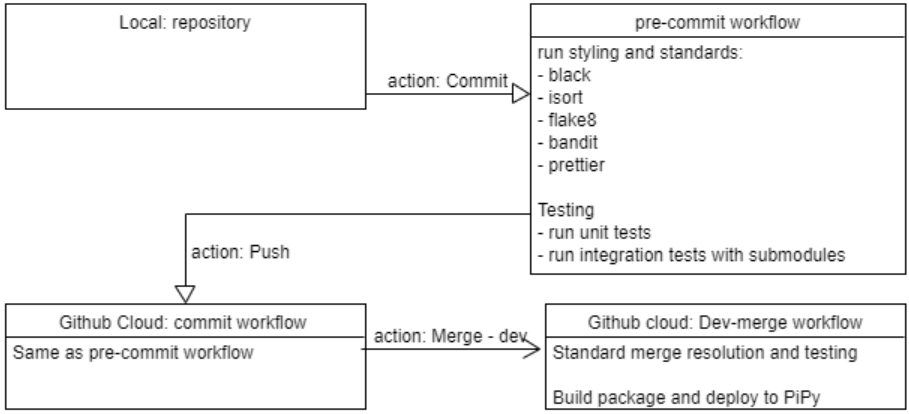
\includegraphics[width=\linewidth]{images/architecture/git-flow}
    \caption{development workflow in git.}
    \label{fig:git-flow}
\end{figure}
\newpage
We followed the agile development process focusing on delivering incrementally and ensuring code is tested and well maintained. To support this we set up a delivery pipeline as seen in figure \ref{fig:git-flow}. We used common tools to ensure python development standards were followed. Black is a code formatting engine ensuring that code looks the same regardless of the programmer. Black enforces a code style transparently and is used by a large number of open source projects and communities. Isort ensures that imports are sorted correctly, preventing Houdini style occurrences of imports mid-way through a file. Flake8 ensures conformance with the PEP8 standard, this includes preventing occurrences of unused imports, and common python programming malpractice such as using\(==\) instead of \(is\) in certain situations. Although most likely unnecessary we decided to include Bandit, a tool designed to find common security issues in python as well. Finally we use prettier to format code automatically in order to make our lives easier when conforming to bandit styling, this allows developers to program in their desired environment without worrying about maintaining a strict style required by black.

For testing we used standard python unit tests, and added hooks to GitHub on a merge action to ensure all tests are passing before a new version of the package is pushed to PiPy. We followed the TDD style of development when working on main modules in order to ensure functionality is stable and works as expected. When modules interact or become more complex this stave a lot of time. The final stage of our workflow is the delivery of a package to any potential users. We decided to use PiPy a popular hosting platform for delivery of pip packages (the most standard library distribution framework in python).

This pipeline we determined is the minimum setup for any viable project aiming for wider use and future development. The advantages of this pipeline are that it is relatively simple hence little to no maintenance is required once everything is set up. This ensures that not time is wasted on unnecessary dev-ops. Having such a pipeline also ensures that agile development can be practiced effectively as we do not have to worry about large integration tests as the process is very iterative. This pipeline also provides stability which is often lacking when performing research as code often breaks and new approaches are added. There are limitations however, one such limitation is the lack of different environments such as development staging and live, although we determined this is unnecessary at this stage and is easily implemented int he future. Another limitation is the lack of testing across multiple environments and versions, we assumed that libraries must be up to date, which may cause issues as backward-compatibility may be important in some use-cases, especially when integrating with older libraries or projects.
\newpage

\subsection{Scope of objectives}
In this section we will review our objectives for the framework and ground them in reality. We need to analyse what features or functionalities are indispensable and which are of less importance. The purpose of this is to ensure that we do not tackle unnecessary problems that can be resolved by simply scaling the project, i.e. a module may not be viable without a core feature, but will be fine without all non-essential features being implemented to date. Take a calculator for example, each calculator has a given complexity or ability to compute problems at different scales, however if you remove a core module of the calculator (such as the ability to process input from the user) then no matter which calculator you choose none will be useful. This is the challenge when building an MVP (minimum viable product).

Our first objective is support for parsing various domain languages to a python standard. We have explored in our related work section that previous work has been attempted, but with little success meaning it will not be viable for our platform. for this reason we have decided to build a parser and translator to python from scratch. As PDDL has evolved we have decided to start with the most basic version and add to it iteratively, this way if we don't complete support for a higher version, we will still have a lower version we can rely on. We are targeting PDDL 2.2 with full test coverage on both the parser, transformer and python representation. We decided to go with PDDL due to the problems we were already working on and it's popularity amongst the planning community. Secondly we want to ensure that we provide an interface layer so that other languages may be supported in the future. If time permits it we may interface a second language if an existing parser exists.

\begin{figure}[h]
    \centering
    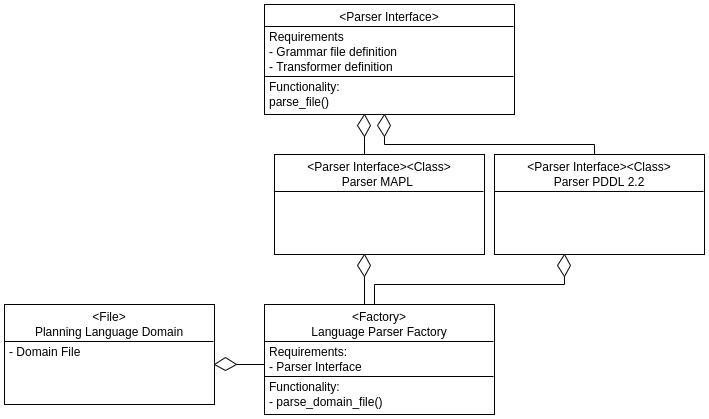
\includegraphics[width=1\linewidth]{images/architecture/parser_uml}
    \caption{Basic parser functionality requirement UML.}
    \label{fig:parser-uml}
\end{figure}
\newpage
Our second objective is to support generation of training data. Here we face our first issue. Training data for planning comes in many formats hence we must define an acceptable standard which is flexible enough to support current development of planning algorithms and maximises existing data generation techniques. We decided that we do not need to place much focus on actual data generation scripts as these are widely available and provide required data-sets in various formats, sizes and languages. We will instead focus on making it as simple as possible to add any existing script for data generation and integrating it with our platform for users to take advantage of. Integration will also involve standardising output format of such scripts. We will be adding several widely available scripts for initial use. This task is not very complex as a lot already exists.
\begin{figure}[h]
    \centering
    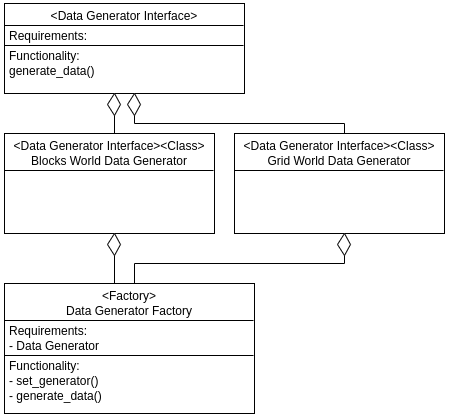
\includegraphics[width=0.7\linewidth]{images/architecture/data_generator_uml}
    \caption{Basic data generation requirement UML.}
    \label{fig:data-generator-uml}
\end{figure}


The third objective is "Simplified implementation of learning models".
This was set in order to make sure that when new users attempt to extend or add new learning models, the rules and requirements to do so are clear and simple to follow.
Hence our scope for this objective is to provide an implementation of an existing learning model (Markov Logic Networks) as well as the abstract classes, to ensure future expandability is guaranteed. We will compare the integration time of the exisitng learning model with our framework with the work done by other papers of similar complexity to generate results.
We aim to make sure that our implementation is decoupled from the framework as a showcase of how one might use with the framework.
We will not be adding multiple learning models as such models compatible with python are not widely available for the precise reason that research code is often missing or broken, hence integrating an existing implementation is an intensive process if one is not familiar with the work.
We have included the architecture diagram displaying how a custome learning model would be integrated \ref{fig:learning-model-uml}
\begin{figure}[h]
    \centering
    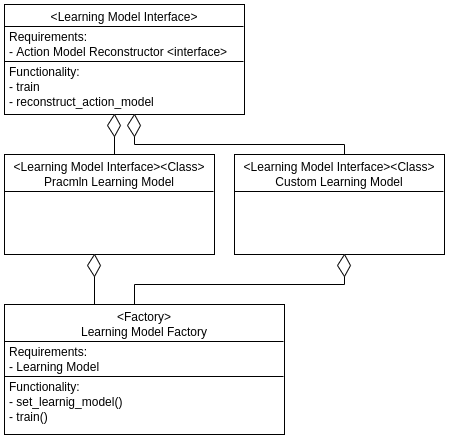
\includegraphics[width=0.7\linewidth]{images/architecture/learning_model_uml}
    \caption{Basic learning model integration UML.}
    \label{fig:learning-model-uml}
\end{figure}

The fourth objective involves the implementation of extendable modules for conversion of training output to a standard action model. We came to the conclusion that these modules are specific to the learning model output hence methods we use for conversion will be proprietary. However our objective is to make it possible for different learning techniques that have the same output to be able to share an action model reconstruction module. This means each module must make it's input data clear to potential users, Python supports typing and we can use documentation to enable such work. We made the decision to provide two action model reconstruction modules in order to demonstrate the use cases these satisfy. A generated action model must be compatible with our simulation module hence for now output is restricted to the only supported language PDDL.
\begin{figure}[h]
    \centering
    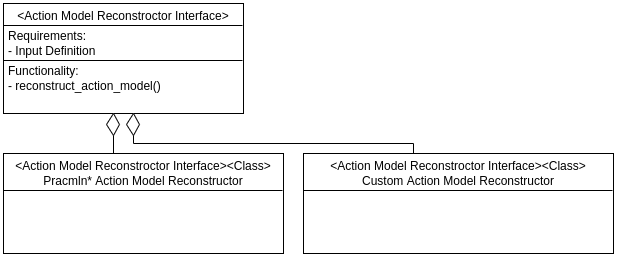
\includegraphics[width=0.7\linewidth]{images/architecture/action_model_reconstructor_uml}
    \caption{Basic action model reconstructor implementation UML.}
    \label{fig:action-model-reconstructor-uml}
\end{figure}
\newpage
The fifth objective is developing a testing framework for learned action models. We will create a python based simulation module taking the learned action models as input and some test data for simulation of the reconstructed action models. We will base the simulator on rules taken from PDDL 2.2 planners. Our objective for the simulator is to generate data and compare data between differently generated action models. We will make such a simulator as modular as possible allowing for simulators written in other languages to be used as well if they exist. Work on simulation has been done, however we deem it important to provide our own as the work is necessary either way if we are translating a planning definition language into python.
\begin{figure}[h]
    \centering
    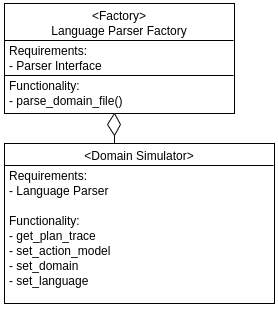
\includegraphics[width=0.4\linewidth]{images/architecture/domain_simulator}
    \caption{Basic action model reconstructor implementation UML.}
    \label{fig:domain-simulator-uml}
\end{figure}

The figures we have presented provide the minimum scope we wish to satisfy for each module, hence they are to be taken as an indicator rather than a full fledged design implementation. We have not provided the full interaction between modules or their full design specification as that will only complicate the ideas we are communicating.

The sixth and final objective is User-friendly and modular adoption of the framework.
For this objective we have decided to follow the same approach that most model ML libraries have adopted.
The idea is to release a python package similar to one such as Tensorflow, and expose each of our modules for the user's benefit.
The reasoning behind this approach is that users will be able to use our framework for projects that have little to do with action model reconstruction.
As we support parsing PDDL and simulating domains, tasks such as writing a PDDL solver or integrating with an ML library can be done directly in python without worrying about interpreting the domain files, this is similar to how pandas allows users to load a CSV file into a DataFrame object, we provide the user with the ability to load a Domain or Problem file into their respective data structures and apply operations over them.
The reasoning behind this approach is that if users determine that these modules are helpful, they will report issues and contribute towards their development, keeping these modules separate ensures that each user can cater the platform and their contribution to their requirements.

A sample project similar to a Jupyter project will be included in the repository, using each module to load a sample domain, generate a dataset of problem states and solutions, and finally train and evaluate a model.
This will be an initial entry point and documentation for any user willing to try using the framework.


\newpage
% 
% sections: Problem Scope


\section{Minimum use-case}
% In the next section we will discuss the baseline for evaluation. We are defining the minimum use-case of the framework that will demonstrate its capability in a given scenario. 

\subsection{Defining baseline objectives}
In order to test the viability of our framework we must define a sample implementation that reflects a vertical slice including all functionality available.
This use-case must reflect the functionality that a student or researcher in the field would require when working on planning problems.
This will provide enough evidence to compare the difference in workload between using our framework and proceeding without. Our aims are as follows:
\begin{enumerate}
    \item Design and generate a database for training a Markov Logic Network, leveraging available domains, problem generators and solvers.
    \item Train a Markov Logic Network.
    \item Evaluate the accuracy of the network given different noise levels.
    \item Reconstruct action models from the trained network.
    \item Compare the reconstructed model with their original counterparts
\end{enumerate}
We can argue that the above steps are common when working on any learning model, most research time may be spent on developing the model itself, however evaluation and analysis is also imperative as new methods need to be compared with existing ones. These steps are useful because they will demonstrate the effect of having a support framework when it comes to menial tasks such as data collection.

The limitations of such a baseline is that it does not expose the framework to enough use cases, it is difficult to gauge the impact of what we have developed based on only one sample implementation. This will only be resolved after wider adoption. As users adopt the framework, unseen issues in the architecture will surface and have the opportunity to be resolved.



% TODO: Formal definition of data we wish to collect

% We discuss the advantages and limitation of our baseline and an outline of general issues that needed to be answered before implementation. We also need to define the output format of results and their credibility. 

\newpage
\section{Analysis}
In this section we define the scope and format of data which we would like to collect to ensure that we can draw satisfactory conclusions from it.
This includes data we require for ensuring the implementation of our learning algorithm is viable, and the data required to gauge how much work went into integration with the framework and how useful our resulting implementation would be for the average user in comparison to other commonly existing implementations.

With respect to the framework, we can use some industry standard metrics for evaluating code/software quality.
The metrics chosen are as follows:

Reliability.
This reffers to the robustness of the software produced, how long can in run without crashing and how many defects are there in the codebase.

Maintainability.
Is the software difficult to maintain?
This can be determined by analysing code complexity, structure, size and consistency.
Various automated tools are available such as Codescene, which provide real values to these metrics using various automated analysis tools.

Testability.
This metric represents how much test coverage there is over the software produced, and what tests other than functional are being run.
Many layers of testing exist, such as functional, smoke,  unit, integration and end-to-end tests are just some of these.
Our aim is to cover which layers we have included, and the reasons for doing so, as well as provide the relevant data on coverage.

Portability.
It is associated with how many environments can adopt the codebase and take advantage of it.
Higher portability is often preferred as it means there is less overhead when adopting the code.
A good example of a highly portable software product is Docker, it allows code to be run in any environment using os-level virtualization.

Reusability.
Checks if the code written can be reused.
This is often the case with decoupled and modular systems.
An example could be how a system managing user accounts can be re-used accross multiple products provided by a single company as functionality is most likely the same.
It is important to design code with reusability in mind as it allows the open-source community to improve smaller modules which individual users take interest in.


With respect to users of the framework, we chose the following metrics:

Adoption Friction.
It represents the barrier that users face when trying to adopt the software.
A simple example with respect to the Planning field would be how the lack of a PDDL to Python parser prevents a user proficient in python from experimenting with PDDL.
An example of the effort that the planning community has gone through in order to reduce the barrier is providing the rules for parsing the PDDL Language.
Our aim is to reduce the Adoption Friction users will have with adopting the use of our platform.
Why should a researcher already using a custom environment switch to using our platform?

Learning Curve.
This refers to how difficult it is for a third-party to start being productive with the software we provide.
We strive to minimise the Learning Curve by leveraging complexity and providing well documented examples.
A low learning curve means that new users with little understanding of fundementals will be able to adopt powerful tools that would otherwise take years to understand their theory.
An example would be the ease of training a CNN using Tensorflow as a user can copy paste widely available examples and simply experiment with different numbers.

Development Complexity.
We included this metric because we want to ensure that no matter the level of user adopting the framework, the LOC (lines of code), and Cyclomatic complexity remains as low as possible.
This ensures that projects involving users that are not well versed in software engineering practices are able to use the framework in a safe and scalable way, whilst maximising legibility.

%TODO wrap things together?
% \subsection{Defining our use-case}

\chapter{Design and Implementation}
In this chapter we will review in detail the design of our framework and each corresponding module.
We will discuss how modules interact and the reasoning behind the design choices we made.
We will also discuss problems which we encountered when building the framework as well as those that came to light during initial use.
We broke down this chapter into sections stemming from the higher level design concepts into the lower level modules.
This will make it easier to piece together the utility of each module we introduce and its required functionality.
After the sections on the framework itself, we will implement our learning algorithm (MLN).
Finally we will review the process of integrating our learning algorithm with the framework and test its overall functionality.
Results and analysis will be reviewed in the next chapter.
% section{What we are doing}
\section{High level architecture}
Before defining the high level architecture for a platform meant to support the development of learning models, we must review what a common learning architecture looks like.
These are well established, and for our system it represents the core of what needs to be supported in order for the framework implementation to be a viable asset to the community.
This includes architecting for the support of different domains, languages and environments as these core components will later be expanded.
A base learning architecture has three components, input data a learning model and an evaluation tool.
In the case of learning action models, input data can be produced from real or synthetic measures, the learning model will need to output an action model, and the evaluation tool will then use a domain simulator to test the action model for validity and accuracy.
A domain simulator can also in turn be used to produce synthetic data.

\begin{figure}[h]
 \centering

 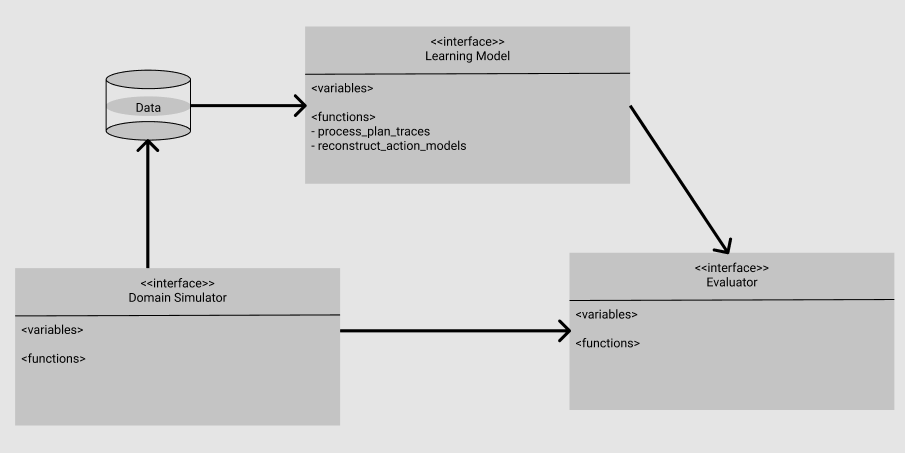
\includegraphics[width=0.7\textwidth]{images/architecture/Core Architecture}
 \caption{Core elements of a learning architecture for reconstructing action models.}

\end{figure}
\newpage
\section{Domain parsing and simulation modules}
\subsection{Parsing module}
For parsing domain languages we implemented the architecture defined in figure \ref{fig:parser-uml}.
Then we proceeded to integrating support for PDDL 2.1 .
The parsing toolkit of choice was Antlr because factors such as ease of use and compatibility with multiple languages made it much easier to develop with.
We could also easily separate a language features/nodes into different files meaning that maintenance and extension of our implementation is much simpler even for people unfamiliar with the structure of modern parsing toolkits.
We followed the BNF Description of PDDL 2.1 defined in \cite{pddl21:online} to ensure compliance with standards.
This also made it easier to test and ensure parsing of each definition was performed correctly.
\begin{figure}[h]
 \centering
 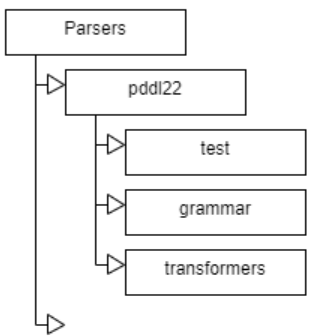
\includegraphics[width=0.3\textwidth]{images/architecture/parser_dir}
 \caption{Directory structure under framework root for integrating parsers.}
  \label{fig:parser-dir}
\end{figure}
\newline
Figure \ref{fig:parser-dir} demonstrates how the integration of new parsers to the framework is done.
We omitted creating an interface layer for transformers with our simulation module as it is unnecessary when working with a single language, and we are interested in an initial proof of concept.
An interface layer was also introduced in order to support for other domain languages in the future, making development much more straight forward.

As of now we based the simulation engine on the semantics defined for the PDDL 2.1 \cite{pddl21:online}.
Rules are extensively defined, and we made sure to separate these in our code allowing for modifications when upgrading for newer versions of PDDL.
Unfortunately this does mean that as of now we have coupled our simulation engine with our parser, however this is only due to the lack of development time invested in this section of the framework.
The disadvantages of this coupling will be evident when attempting to integrate a new parser, as it will have to follow the rules of the engine.
However we do assume that this can be mitigated over time by upgrading and extending the simulation engine to support different input formats and rules therefore making it more generic.
\newpage
To provide an indication of how the parser is implemented we will now provide a vertical slice of a simple lexical component.
Our example will be on the implementation of the predicate in the PDDL 2.1 specification.
The specification states that the predicate is defined as follows:
\begin{lstlisting}
<predicate>     ::= <name>
*** dependencies ***
<name>          ::= /([a-zA-Z]|\d)+((_|-)([a-zA-Z]|\d)+)*/
\end{lstlisting}
With this specification we can define the grammar.lark file for predicate, we assume that all dependencies are satisfied.

\begin{lstlisting}t
%import .name.name

predicate: name
\end{lstlisting}
This demonstrates how simple our chosen architecture is and how flexible the system is to modify. The next step is to specify the transformer that converts predicate nodes into a python data structure for use in the simulator.

\begin{lstlisting}[language=Python]
from lark import Transformer


class Predicate(Transformer):

    @staticmethod
    def predicate(args):
        val = args[0].children[0]
        return val

\end{lstlisting}
Predicate is a relatively simple structure so we only need to recover the stored underlying value of "name" as they are both strings, more complicated structures such as actions, depend on more complex implementations that align with their use cases.
Finally we test the parser to ensure that it performs as expected given the data we would reasonably expect to pass it:


\newpage
\begin{lstlisting}[language=Python]
import os
from unittest import TestCase
from lark import Lark
from pddl_parser.transformers import Predicate

class TestGrammarPredicate(TestCase):
    def setUp(self) -> None:
        self.grammar = """
        start:predicate
        %import .predicate.predicate
        %import common (WS)
        %ignore WS
        """
        self.transformer = Predicate()
        self.import_path = [f'{os.getcwd()}/../../grammar/']
        self.parser = "lalr"

    def test_predicate_parses_kebab_case(self):
        try:
            parser = Lark(grammar=self.grammar, import_paths=self.import_path, parser=self.parser)
            parser.parse("""predicate-with-dashes""")
        except Exception as e:
            self.fail(msg=e)

    def test_predicate_parses_snake_case(self):
        try:
            parser = Lark(grammar=self.grammar, import_paths=self.import_path, parser=self.parser)
            parser.parse("""predicate_with_underscores""")
        except Exception as e:
            self.fail(msg=e)

    def test_predicate_parsing_fails(self):
        parser = Lark(grammar=self.grammar, import_paths=self.import_path, parser=self.parser)
        self.assertRaises(Exception, parser.parse, """space separated""", msg='failed to raise on space separator')
        self.assertRaises(Exception, parser.parse, """(not-char""", msg='failed to raise on non char in word')
        self.assertRaises(Exception, parser.parse, """1not-num""", msg='failed to raise on num in word')

    def test_predicate_transformer(self):
        try:
            parser = Lark(grammar=self.grammar, import_paths=self.import_path, transformer=self.transformer,
                          parser=self.parser)
            parser.parse("""predicate-with-dashes""")
        except Exception as e:
            self.fail(msg=e)
\end{lstlisting}
We can observe that tests are more extensive as we want to ensure that when using our parser unwanted behaviour does not occur.
Code is only ever as good as the tests supporting it because when modifications are made, only tests can assure a developer that other features have not been compromised and if they have, then there are clear steps to fixing them.

\subsection{Simulation module}
The simulation module relies on being populated by an initial state conforming to a json standard as of now defined by the Parsing module.
A domain is parsed and converted to a json representation which is easier to manage.
Actions are then initialised from the parsed domain and an initial state is populated from a parsed problem file.
The simulator at this time permits the execution of actions and the tracking of changes in the state.
This functionality although relatively rudimentary has been sufficient for the purpose of producing plan traces and verifying if simple actions performed correctly when generated by the learning model.

\begin{lstlisting}[language=Python]
class State:
    def __init__(self, state:dict):
        self._actions = dict()
        self.actions = state["actions"]
        self.state = set()
        self.latest_removed = set()
        self.latest_added = set()
        # self.latest_added=set()

    @property
    def actions(self) -> dict:
        """
        Actions that can be performed on the domain state.
        """
        return self._actions

    @actions.setter
    def actions(self, actions: list):
        """
        Setter for actions of the state, must a list of json dictionaries.
        """
        for a in actions:
            self._actions[a["name"]] = Action(**a)

    def perform_action(self, p: Predicate):
        """
        Perform an action in the format of Predicate ( "name(*v)") on the state.
        :raises KeyError if action does not exist.
        """
        pos = self.actions[p.name].get_pos_list(p.args)
        self.state = self.state | pos
        self.latest_added = pos
        neg = self.actions[p.name].get_neg_list(p.args)
        self.latest_removed = neg
        self.state = self.state - neg

    def set_init_state(self, predicate_json):
        """
        Populates initial states with predicates
        """
        for p in predicate_json:
            self.state.add(Predicate(**p))
\end{lstlisting}

The above is a simplified version of the Simulation module, it provides a bare-bones PDDL action simulator.
As problems become more complex and simulation needs to support more functionality, this module can be expanded and eventually integrated with third-party tools such as Unity (for simulating 3d models) or Gazebo with ROS (robot operating system) to view how a state changes in real time.
Performing an action and testing if a goal state has been reached is very intuitive which is helpful for legibility and use.


\newpage

\section{Learning model interface and implementation}
The learning model interface defines the class interaction that is required for the full implementation of a learning model.
We are only displaying the UML nearest neighbours as previously mentioned in order to best demonstrate the functionality required by the module we are working with.
\begin{figure}[h]
 \centering
 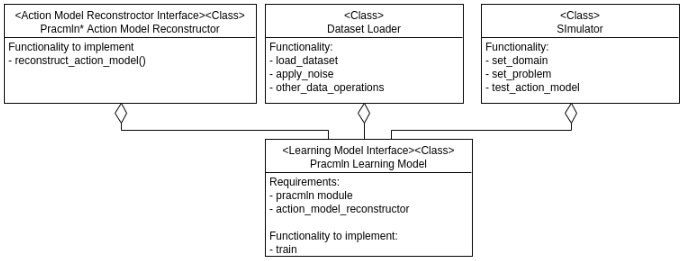
\includegraphics[width=1\textwidth]{images/architecture/learning_module_interaction_uml}
 \caption{Learning model class dependency UML.}
  \label{fig:learning-module-interaction-uml}
\end{figure}
\newline
The above figure displays how we have implemented a sample learning model.
For the implementation of the train function we have full use of the dataset loader to get the necessary data and perform any transformation on it.
The dataset loader is similar to a library like Pandas, providing the ability to load data in the correct format from files.
This was a necessary implementation in our use case are defined differently from standard numpy arrays.
We previously defined the data generation interface, this interface ensures that data is compatible with our dataset loader and is flexible enough for any use by the implemented learning model.
The learning model can also make use of the simulator to test if the predicted action model is valid and how well it performs on given problems.
This can be used as part of the optimization function when training, although we have tested this to date.

The code associated with this module is provided to the user under name of "learn".
The base interface as of this moment is as follows:
\begin{lstlisting}[language=Python]
from abc import abstractmethod

class LearningModelInterface:
    def __init_subclass__(cls, **kwargs):
        pass

    @abstractmethod
    def train(self):
        ...
\end{lstlisting}
We can observe that the interface any new learning model classes must conform to is relatively lax.
This approach was taken in order to provide as much freedom to the developer as possible until more robust standards are put in place.
The implementation for the pracmln learning model which we have implemented follows the above specification and is available for public use.
This class signature also provides a familiar interface for users using models in all common ML libraries, the train function is very well known and abstracts the complex inner workings of a learning algorithm away.

Here is our sample implementation for the pracmln learning module using a StateInference object to manage databases and the MarkovNetworks being generated:
\begin{lstlisting}[language=Python]
import os
import random

from collections import defaultdict
from learn import LearningModelInterface
from .state_inference import Database as DB
from .state_inference import StateInfrence
from .utils import load_dbs


class PracmlnLearningModel(LearningModelInterface):
    def __init__(
            self,
            mln_database_path: str,
            domain_p_decs_path: str,
            max_databases=25,
    ):
        # load dataset
        databases = load_dbs(mln_database_path)
        random.shuffle(databases)
        databases = databases[:max_databases]
        self.dataset = [DB.parse_db(db) for db in databases]

        # initiate pracmln learner
        self.state_inference: StateInfrence = StateInfrence(
            os.path.normpath(os.path.join(os.getcwd(), domain_p_decs_path))
        )

    def train(self):
        # track how many databases were added for each action being learnt
        opt_tracker = defaultdict(int)
        for i, d in enumerate(self.dataset):
            # pass data through Markov Logic Network
            self.state_inference.process_database(d)
            opt_tracker[d.action.name] += 1
            # write data for metrics, remove for speed & space use reduction
            self.state_inference.save_data_for_graphing()
        # plot learning confidence results.
        self.state_inference.plot()
\end{lstlisting}
This sample of code provides an example of the freedom provided when developing a custom learning module.
Having the flexibility provided facilitates experimental use and design whilst conforming to a bare minimum of standards which are necessary for legibility and wider adoption.
The simplicity of using this interface will be highlighted when the sample project demonstrated.
The detail for the inner workings such as dataset structure and training of the MLN learning module are specified in the next chapter.

\newpage
\section{Integrating MLN Learner module}
A STRIPS domain consists of a state \(S\) and a set of action models \(M\).
\(S\) is a set of predicates with typed arguments.
A strips action model \(A\) which we are attempting to reconstruct, is defined by  \(\{a,a_{pre},a_{add},a_{del}\}\). \(a\) is the name with typed arguments of the function, \(a_{pre}\) is set of preconditions which specify the conditions of a state under which \(a\) can be applied. \(a_{add}, a_{del}\) is the add and delete list respectively, these lists indicate the effects of \(a\) on a state, specifying which new predicates are to be added and which existing predicates are to be removed.
\newline \newline
We define a valid database \(D\) by \(\{a,S_{p}\}\) where \(S_p\)  is a set of predicates in the form \(p_{name}(p_{args},f\in \{-1,0,1\})\), the modification here is that we have added a variable \(f\) to each predicate representing if it is a member of \(a_{add}\) if \(f=1\), \(a_{del}\) if \(f=-1\) and the set of predicates where \(f=0\) form a super-set of \(a_{pre}\).
\newline \newline
A plan with its intermediate state-action pairs can hence be represented as an ordered list of databases. This representation is useful because it allows us to now create a model which predicts \(A\) given a partially complete database after training.
\newline \newline
In order to tackle possible noise in the database we need to use a model that can handle constraints being violated, one such model is a Markov Logic Netork (MLN). Where as a first-order knowledge base is a set of hard constraints on a set of possible worlds in which a violation of a constraint implies 0 probability for said world. MLN's soften these constraints and reduces the weight of the violating constraint making the world less probable instead of impossible. MLN's are formulated as a set of pairs \(w_i,F_i\) where \(w_i\) is the weight of a formula represented as a real number, and \(F_i\) is a formula in first-order logic. Together with a finite set of constraints \(C = \{c_1,c_2,...,c_{|C|}\}]\), it defines Markov network \(M_{L,C}\) as follows:
%ref: https://homes.cs.washington.edu/~pedrod/kbmn.pdf
% equation 1
% equation 2
\section{Training and reconstruction of STRIPS action models}
Strips action models can be reformulated as a conjunction of typed predicates \(a_{pre},a_{add},a_{del}\), this set of predicates belonging to a specific action should represent a subset of a database for a matching action. As we have no prior knowledge of the valid subset when creating and training the MLN, we must assume that all predicates a valid and generate an MLN accordingly. Once weights reduce bellow a set threshold we can prune them out of the MLN as they represent predicates that would render the action model improbable.
    \newline \newline

The algorithm for generating and training an MLN from a database instance is as follows:

\newline
process \(D\):\newline
\(MLN \impliedby action\_MLNS[a] \) \newline
for each predicate \(p\) that has not been pruned or previously added to \(MLN\):\newline
----- generate and add formula: \(a \implies p\) with initial weight 0 to \(MLN\)\newline
train MLN (online)  with database \(D\)\newline
prune weights (for efficiency)\newline

once training is complete we can extract each predicate with its weight .

An optimization for the above routine is to prune any predicates that does not share variables with the action being processed.

Due to a lack of resources available for working with PDDL in python, I have designed a system for generating generic plan traces from PDDL in python. This was necessary as many modern learning tools use python and it is a language that saves a lot of development time thanks to readily available complex libraries (Tensorflow, Pracmln, Pytorch, Sklearn etc...). Such libraries will allow for more interesting strategies in tackling the problem at hand. \newline \newline
The greatest difficulty encountered is in the Generation of Plan Traces, as planners used don't provide intermediate states or add and delete lists, hence these must be generated from the parsed action models directly. There are no known libraries for parsing action models that support more than simple STRIPS, hence a custom extendable parser was
implemented.


\newpage
\section{Final integration}
\begin{figure}[h]
 \centering
 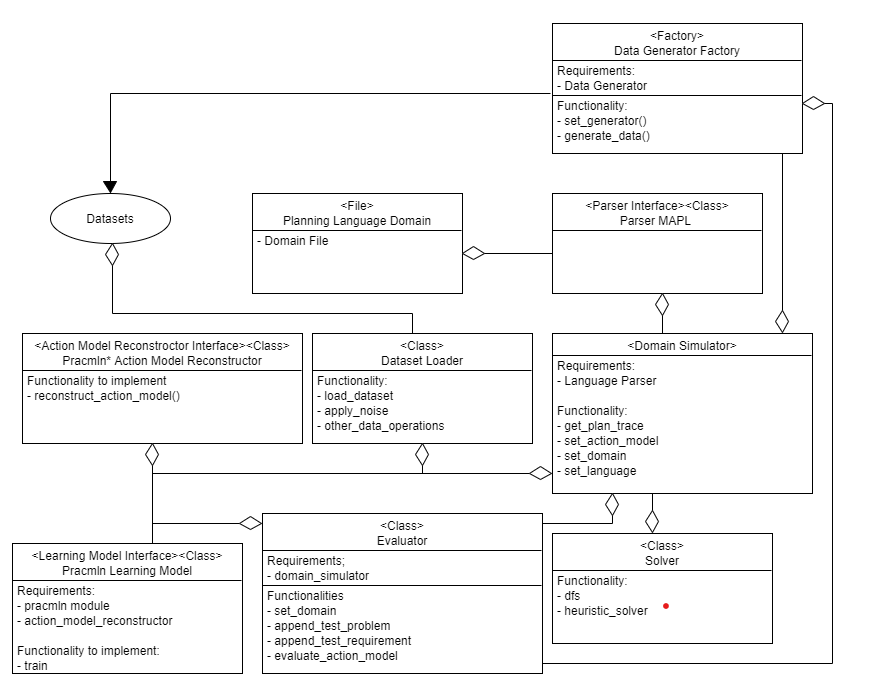
\includegraphics[width=1\textwidth]{images/architecture/final_integration_uml}
 \caption{Relations of most important modules for complete framework for a specific use-case, ignoring interfaces}
  \label{fig:learning-module-interaction-uml}
\end{figure}
In the figure above, we display the interaction between all important modules for our use case. This ignores the interfaces we provided for other languages, domains, data generators and learning models that can be added seamlessly to the framework. We can observe the end to end flow of data, from the initial generation of training datasets, to the training of prediction models and their evaluation.


As all of the necessary modules have now been defined, we can demonstrate a sample project that specifies a specific domain, generates a dataset, trains a model on this dataset and finally evaluates the trained model:

\begin{lstlisting}[language=Python]
import os

from generator.generator import GridWorldGenerator
from solvers.solvers import FFXSolver
from learn.pracmln_learning_model.utils import write_dbs
from learn.pracmln_learning_model import PracmlnLearningModel
from learn.pracmln_learning_model.utils import MLNDeclarationGenerator

BASE_PATH = os.path.normpath(f"{os.getcwd()}/..")

PROJECT_DIR = os.path.dirname(__file__)
DATA_DIR = f"{PROJECT_DIR}/data"
PROBLEM_STATE_DSET_DIR = f"{DATA_DIR}/problem_states"
DOMAIN_FILE = f"{PROJECT_DIR}/grid.pddl"
PROBLEM_SOLUTION_DIR = f"{DATA_DIR}/problem_solutions"
MLN_DATABASE = f"{DATA_DIR}/mln_db.mln"
DOMAIN_P_DECS = f'{DATA_DIR}/mln_grid_p_decs.txt'
# generate problem dataset
GridWorldGenerator.generate_data(output_dir=PROBLEM_STATE_DSET_DIR)
# generate solutions dataset
FFXSolver.solve_problem_dir(
    domain_file=DOMAIN_FILE,
    problem_dir=PROBLEM_STATE_DSET_DIR,
    output_dir=PROBLEM_SOLUTION_DIR,
)
# simulate solutions to generate plan trace dataset (mln_db)
write_dbs(
    domain_file=DOMAIN_FILE,
    problem_state_dir=PROBLEM_STATE_DSET_DIR,
    problem_solution_dir=PROBLEM_SOLUTION_DIR,
    mln_db_path=MLN_DATABASE,
)
# generate necessary mln predicate declarations
MLNDeclarationGenerator.gen(DOMAIN_FILE, DOMAIN_P_DECS)
# instantiate and train model
model = PracmlnLearningModel(mln_database_path=MLN_DATABASE, domain_p_decs_path=DOMAIN_P_DECS)
model.train()
\end{lstlisting}\label{example-project}

From the above code we can observe how comfortable the process is from generating necessary data, simulating a pddl domain state to training a model.
The simplicity and modularity being a key aspect of our design goals can be clearly observed.
An initial dataset of 100 problems is generated for the specified domain.
A specified solver in this case FFX generates a solutions dataset given our problems and domain.
The Simulation module generates plan traces from the solutions and problems and creates a dataset of MLN databases for the learning model.
Finally the learning model processes these databases and traines a markov network for each action present in the dataset.

%  Existing  techniques for learning action traces...

%  define error for preconditions

% extrapolate to error of action model.




% Encoding of action plan trace (Database)

% Encoding of a logic network
% Training of a logic network
% Noise
% Prediction
% Error evaluation

\chapter{Tests and Analysis}
In this chapter we will review the goals set out in chapter 3.3 Analysis and to what extent these have been achieved, where success was observed and where failures occured and what improvements could be made.
We will first review the metrics associated with the framework then with the use of the framework and finally we will review some output produced with our sample project.
\section{Metrics report}
\subsection{Framework - Reliability}
As there is no active use of the framework, the only viabile data for reliability of the framework is our active development and test coverage data.
Framework test coverage is at \(95\%\) code coverage which is respectable.
There are no active bugs currently identified, and non-trivial code contains documentation.


Maintainability.
Is the software difficult to maintain?
This can be determined by analysing code complexity, structure, size and consistency.
Various automated tools are available such as Codescene, which provide real values to these metrics using various automated analysis tools.

Testability.
This metric represents how much test coverage there is over the software produced, and what tests other than functional are being run.
Many layers of testing exist, such as functional, smoke,  unit, integration and end-to-end tests are just some of these.
Our aim is to cover which layers we have included, and the reasons for doing so, as well as provide the relevant data on coverage.

Portability.
It is associated with how many environments can adopt the codebase and take advantage of it.
Higher portability is often preferred as it means there is less overhead when adopting the code.
A good example of a highly portable software product is Docker, it allows code to be run in any environment using os-level virtualization.

Reusability.
Checks if the code written can be reused.
This is often the case with decoupled and modular systems.
An example could be how a system managing user accounts can be re-used accross multiple products provided by a single company as functionality is most likely the same.
It is important to design code with reusability in mind as it allows the open-source community to improve smaller modules which individual users take interest in.


With respect to users of the framework, we chose the following metrics:

Adoption Friction.
It represents the barrier that users face when trying to adopt the software.
A simple example with respect to the Planning field would be how the lack of a PDDL to Python parser prevents a user proficient in python from experimenting with PDDL.
An example of the effort that the planning community has gone through in order to reduce the barrier is providing the rules for parsing the PDDL Language.
Our aim is to reduce the Adoption Friction users will have with adopting the use of our platform.
Why should a researcher already using a custom environment switch to using our platform?

Learning Curve.
This refers to how difficult it is for a third-party to start being productive with the software we provide.
We strive to minimise the Learning Curve by leveraging complexity and providing well documented examples.
A low learning curve means that new users with little understanding of fundementals will be able to adopt powerful tools that would otherwise take years to understand their theory.
An example would be the ease of training a CNN using Tensorflow as a user can copy paste widely available examples and simply experiment with different numbers.

Development Complexity.
We included this metric because we want to ensure that no matter the level of user adopting the framework, the LOC (lines of code), and Cyclomatic complexity remains as low as possible.
This ensures that projects involving users that are not well versed in software engineering practices are able to use the framework in a safe and scalable way, whilst maximising legibility.

\section{Tests}
we can track weights with varying noise in the databases. Systematic noise can be added by removing a target set of predicates with a given probability. And Random noise can be added by removing any given predicate by a defined probability.

Accuracy
We measure accuracy by analysing how similar a derived logic network is to the expected logic network which we can construct. We can calculate the error rate for \(a_{pre}\) by the following formula:
\[E(a_{pre})=\frac{a_{pre}\cap \{p\in MLN_{|(f\in p) =0}\}|}{\max( |a_{pre}|,|p\in MLN|)}\]
The same formula can be applied for \(a_{add},a_{del}\) simply by replacing the 0 with 1 and -1 respectively. The total error of the resulting MLN is the average of the above three errors expressed by the equation bellow.
\[E(MLN)=\frac{sum(E(a_{pre}),E(a_{del}),E(a_{add}))}{3}\]

\section{Tracking weights}
As a preliminary experiment, weights were pruned due to the excessive time it took to train the MLN, this means only the predicates that are related to the action model are being trained.
I have also included the cumulative weights (sum of independently trained MLN's for each database and action model.


\begin{figure}[h]
 \centering
 \begin{minipage}[b]{0.49\linewidth}
 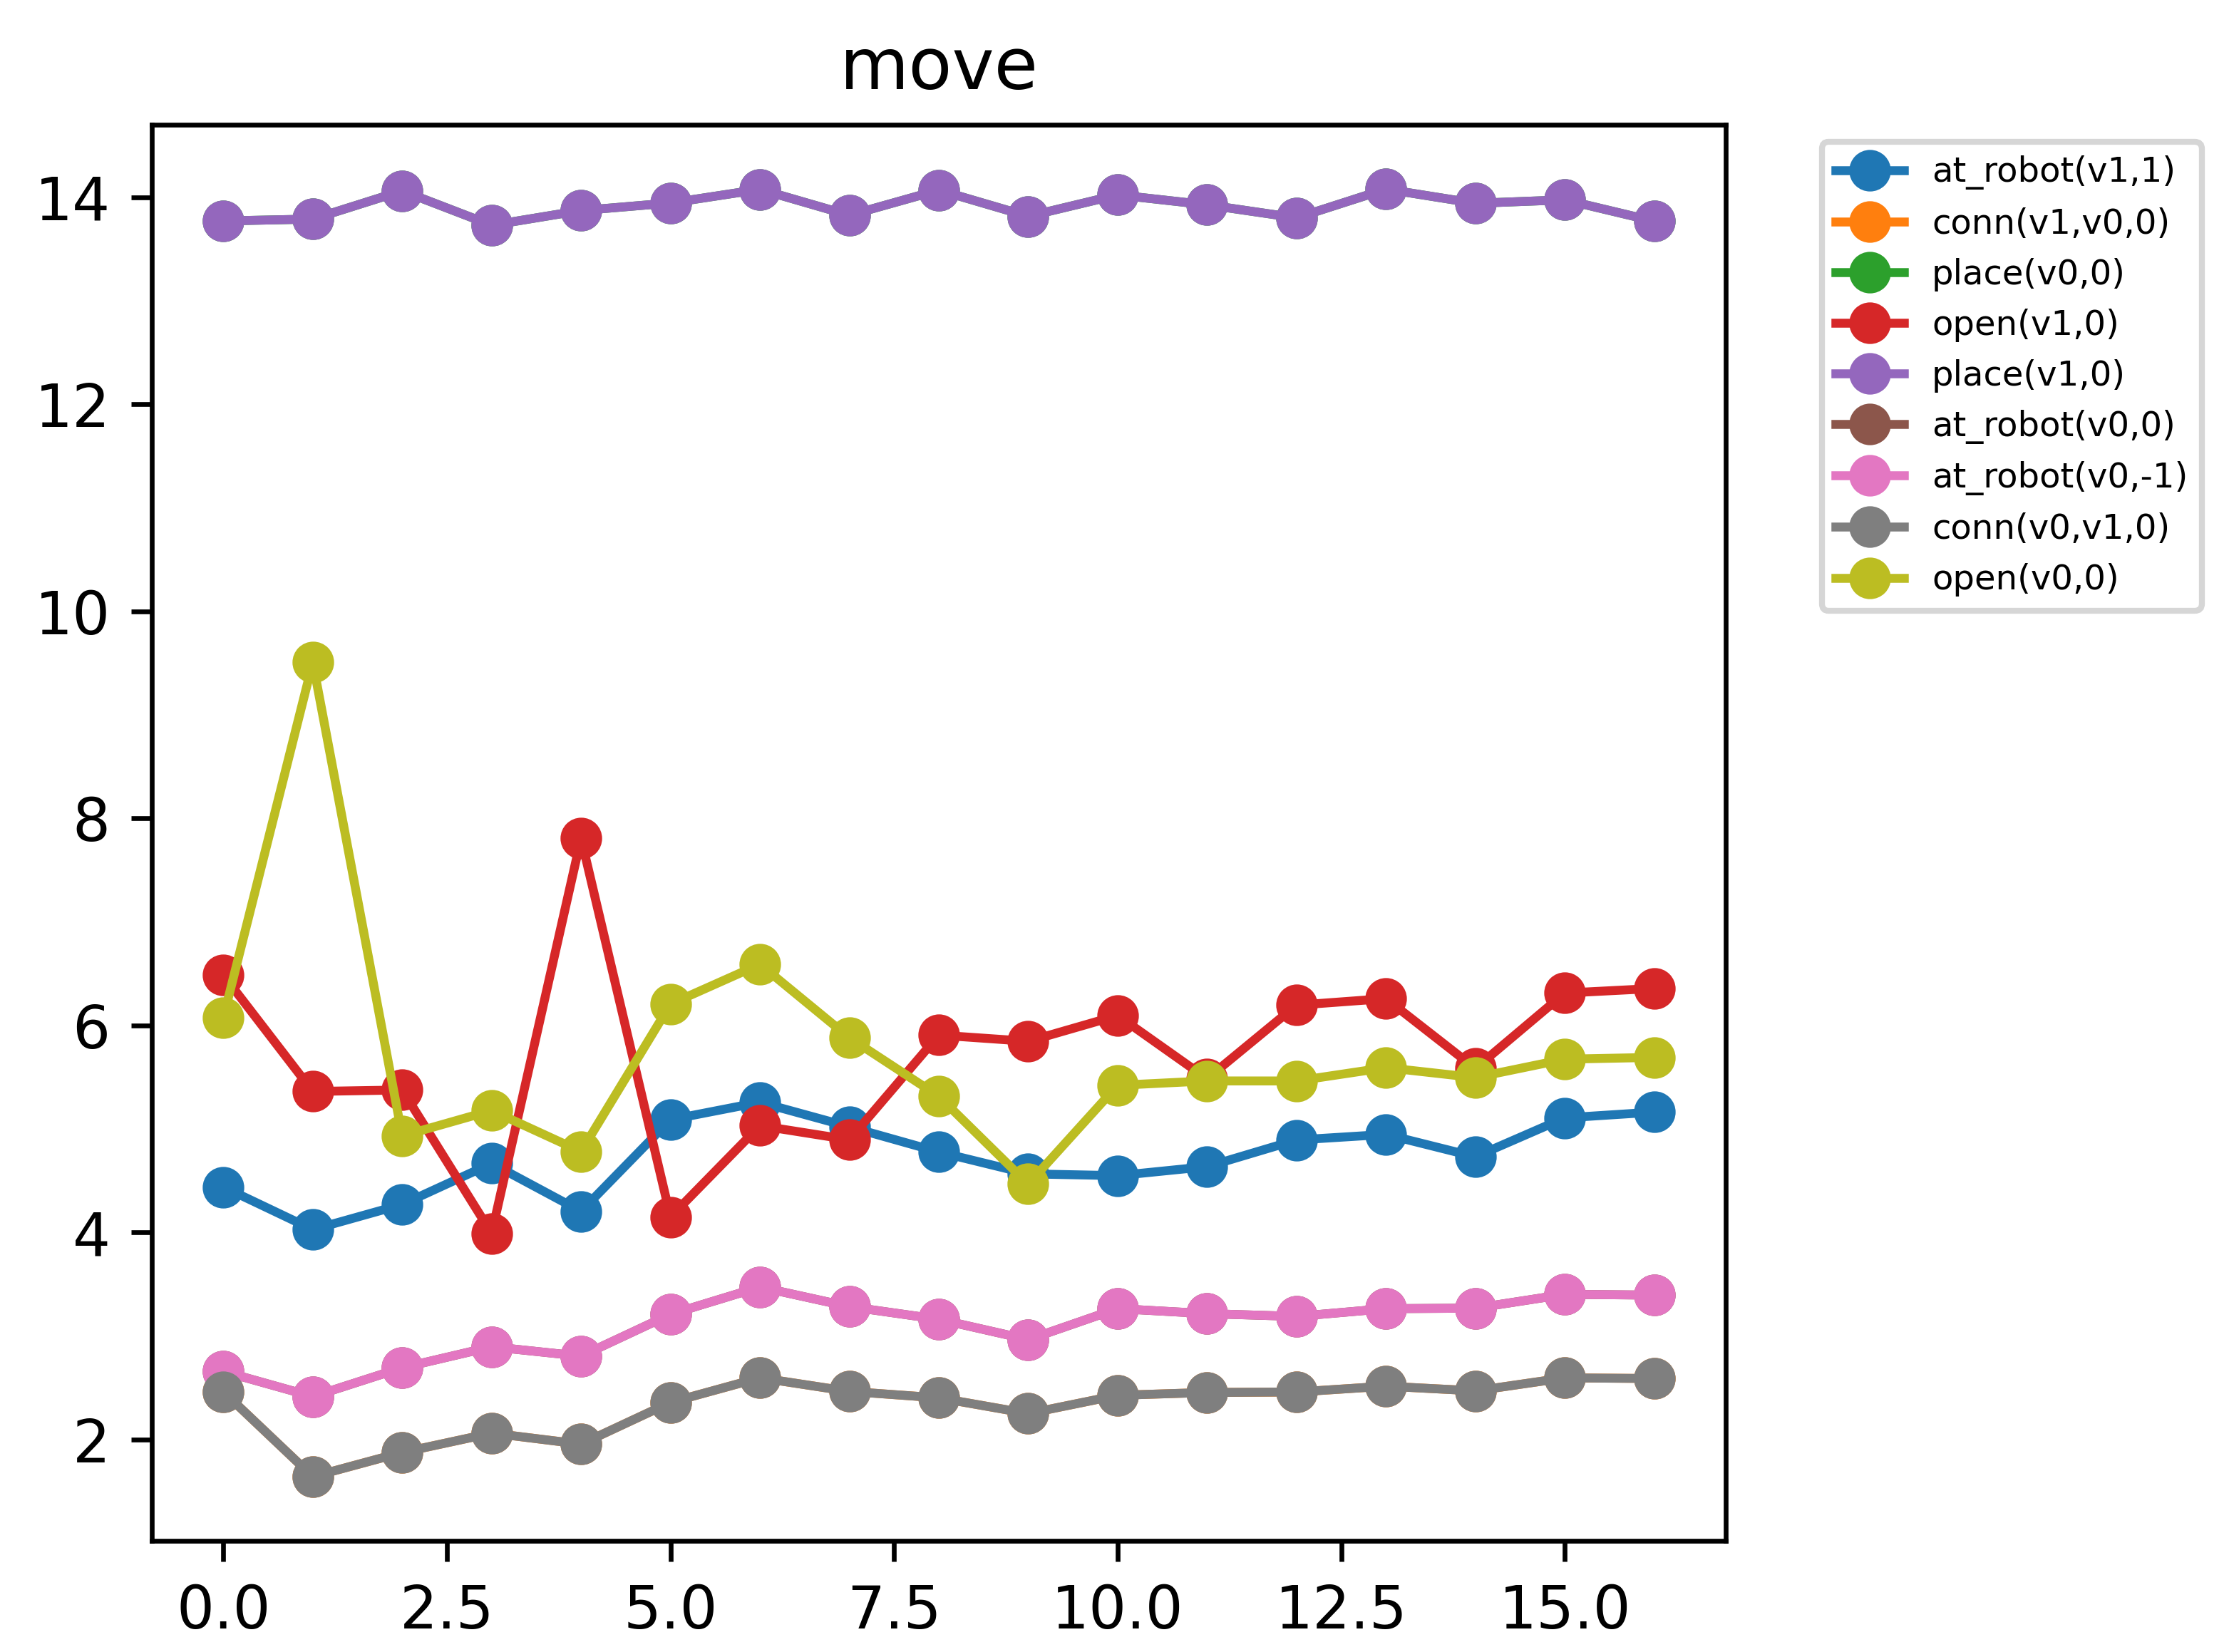
\includegraphics[width=1\textwidth]{images/tests/movegraph_100}
 \caption{Move action MLN, no noise {fig:mv 100}}

 \end{minipage}
 \hfill
 \begin{minipage}[b]{0.49\linewidth}

 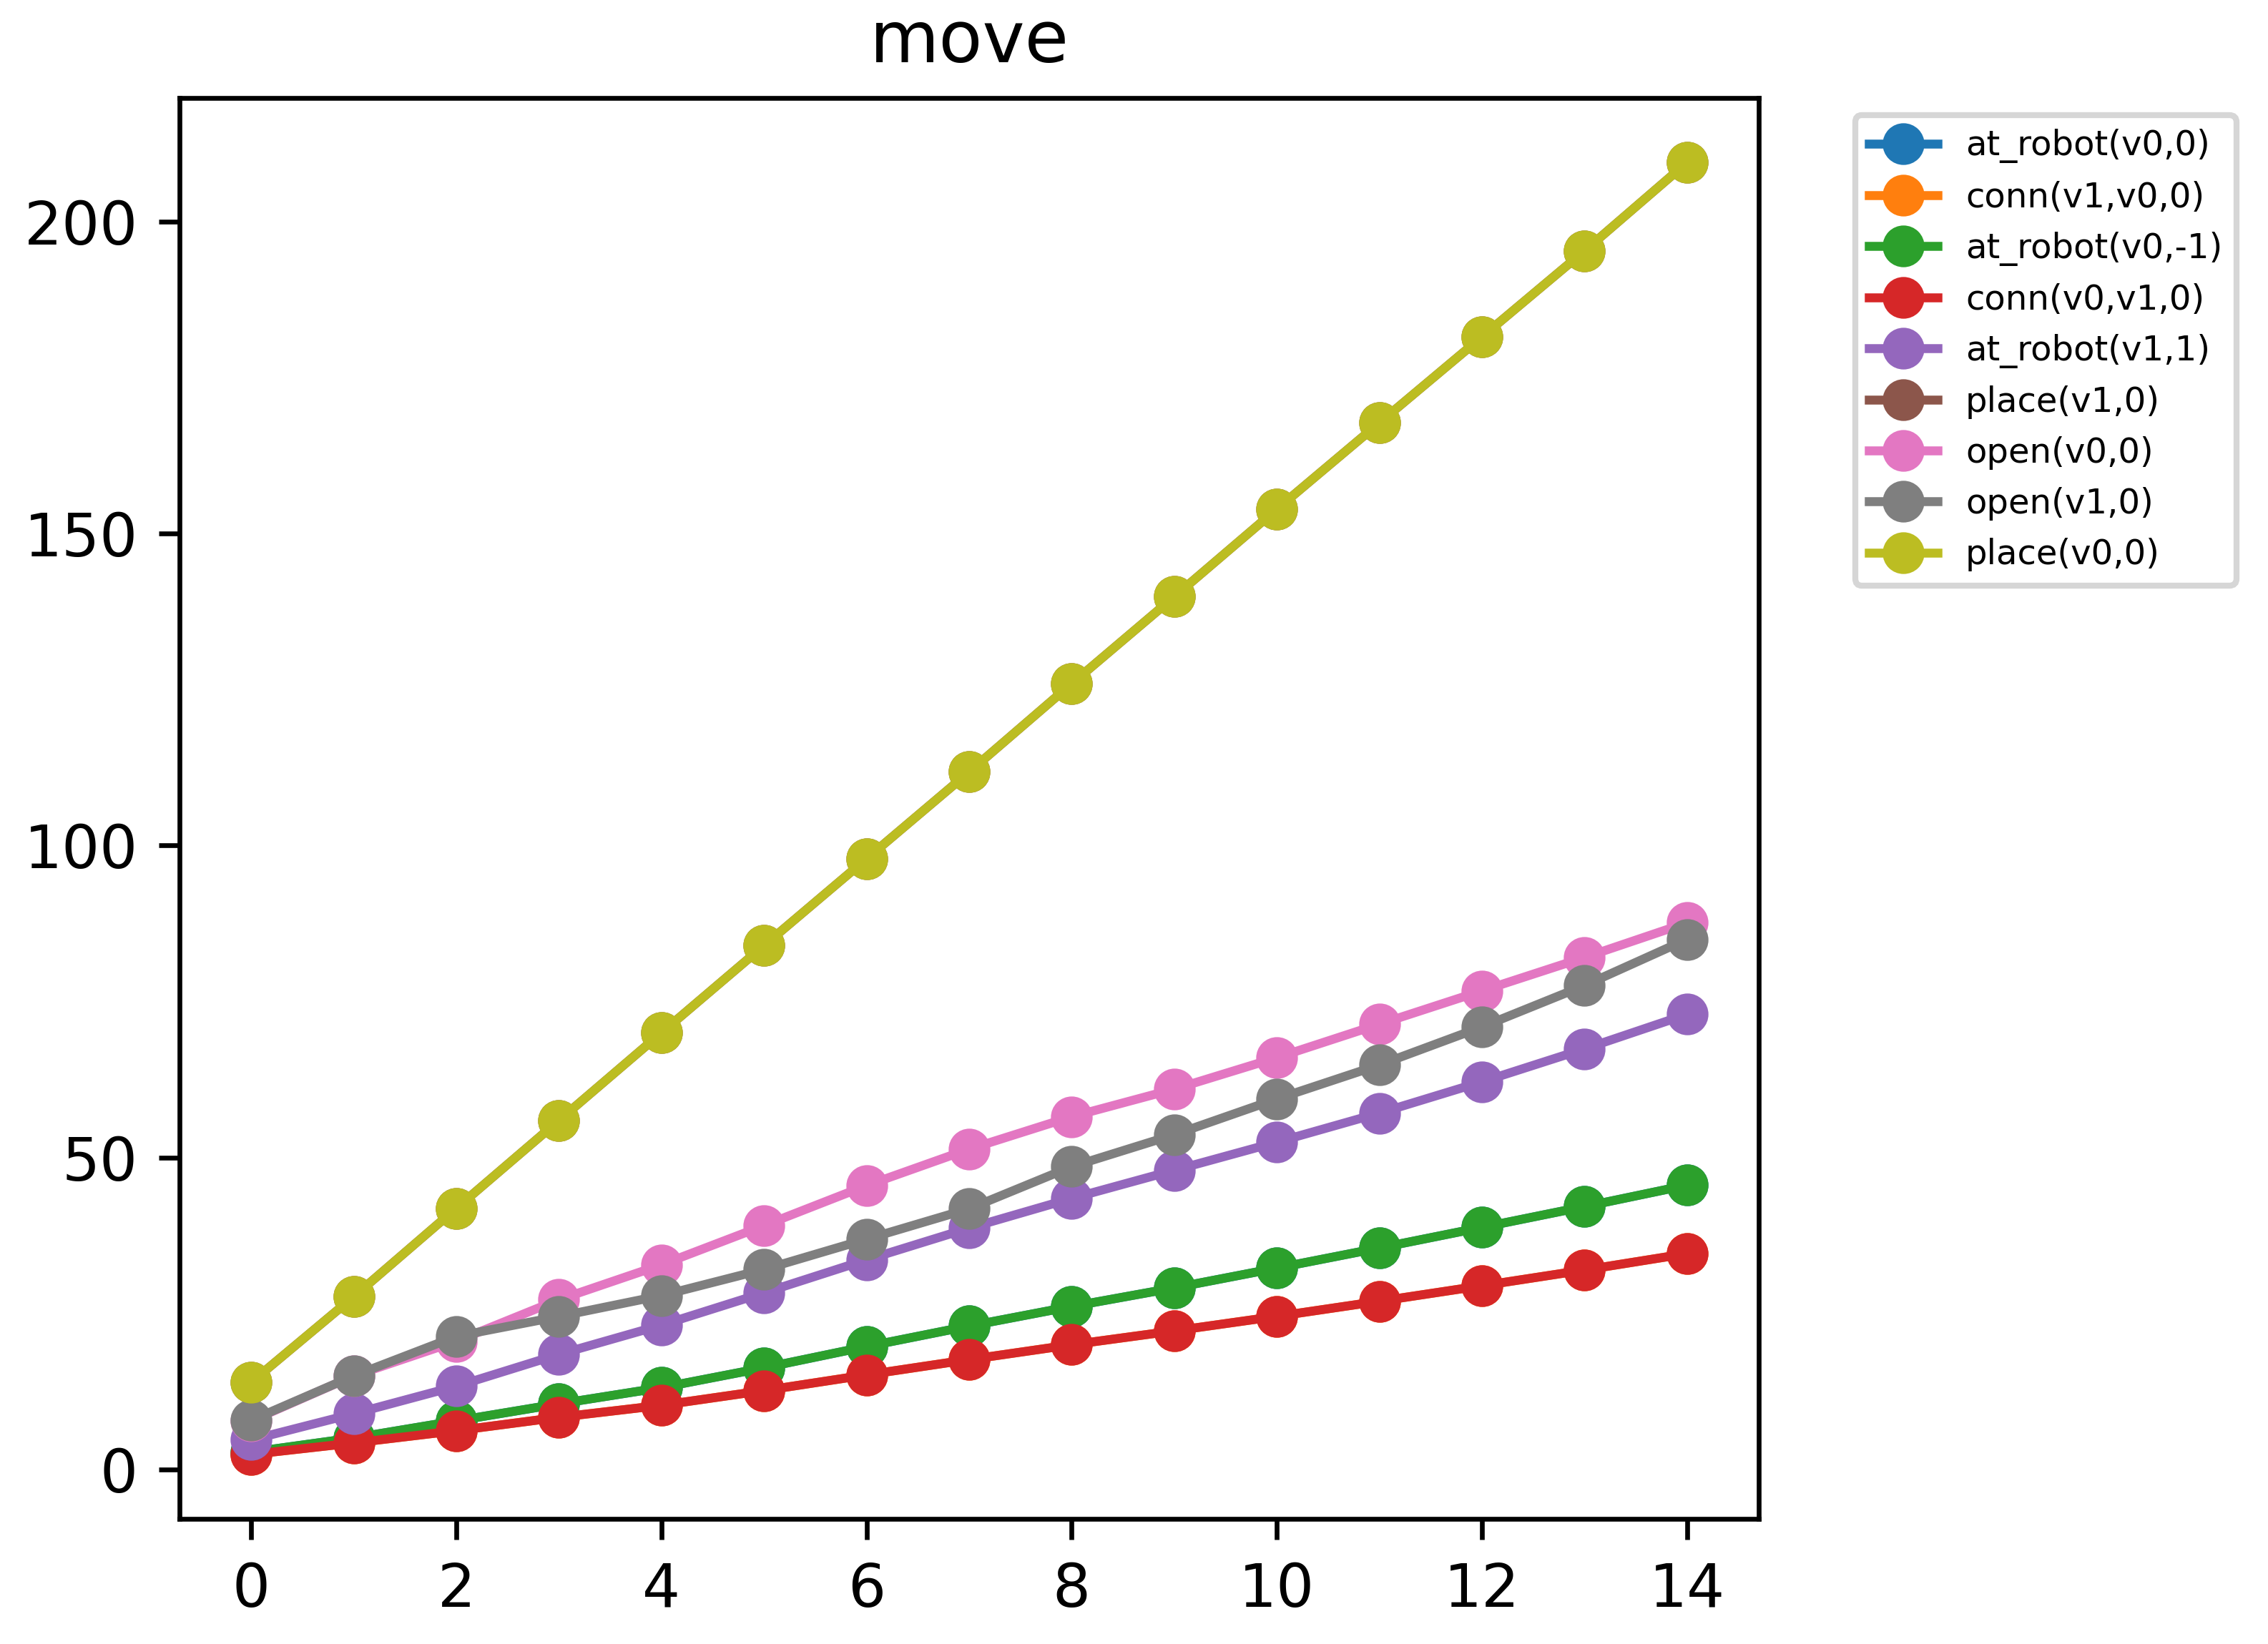
\includegraphics[width=1\textwidth]{images/tests/movegraph_100_cum}
 \caption{Move action MLN (cumulative), no noise {fig:mv 100 cum}}

 \end{minipage}
\end{figure}

\begin{figure}[h]
 \centering
 \begin{minipage}[b]{0.49\linewidth}
 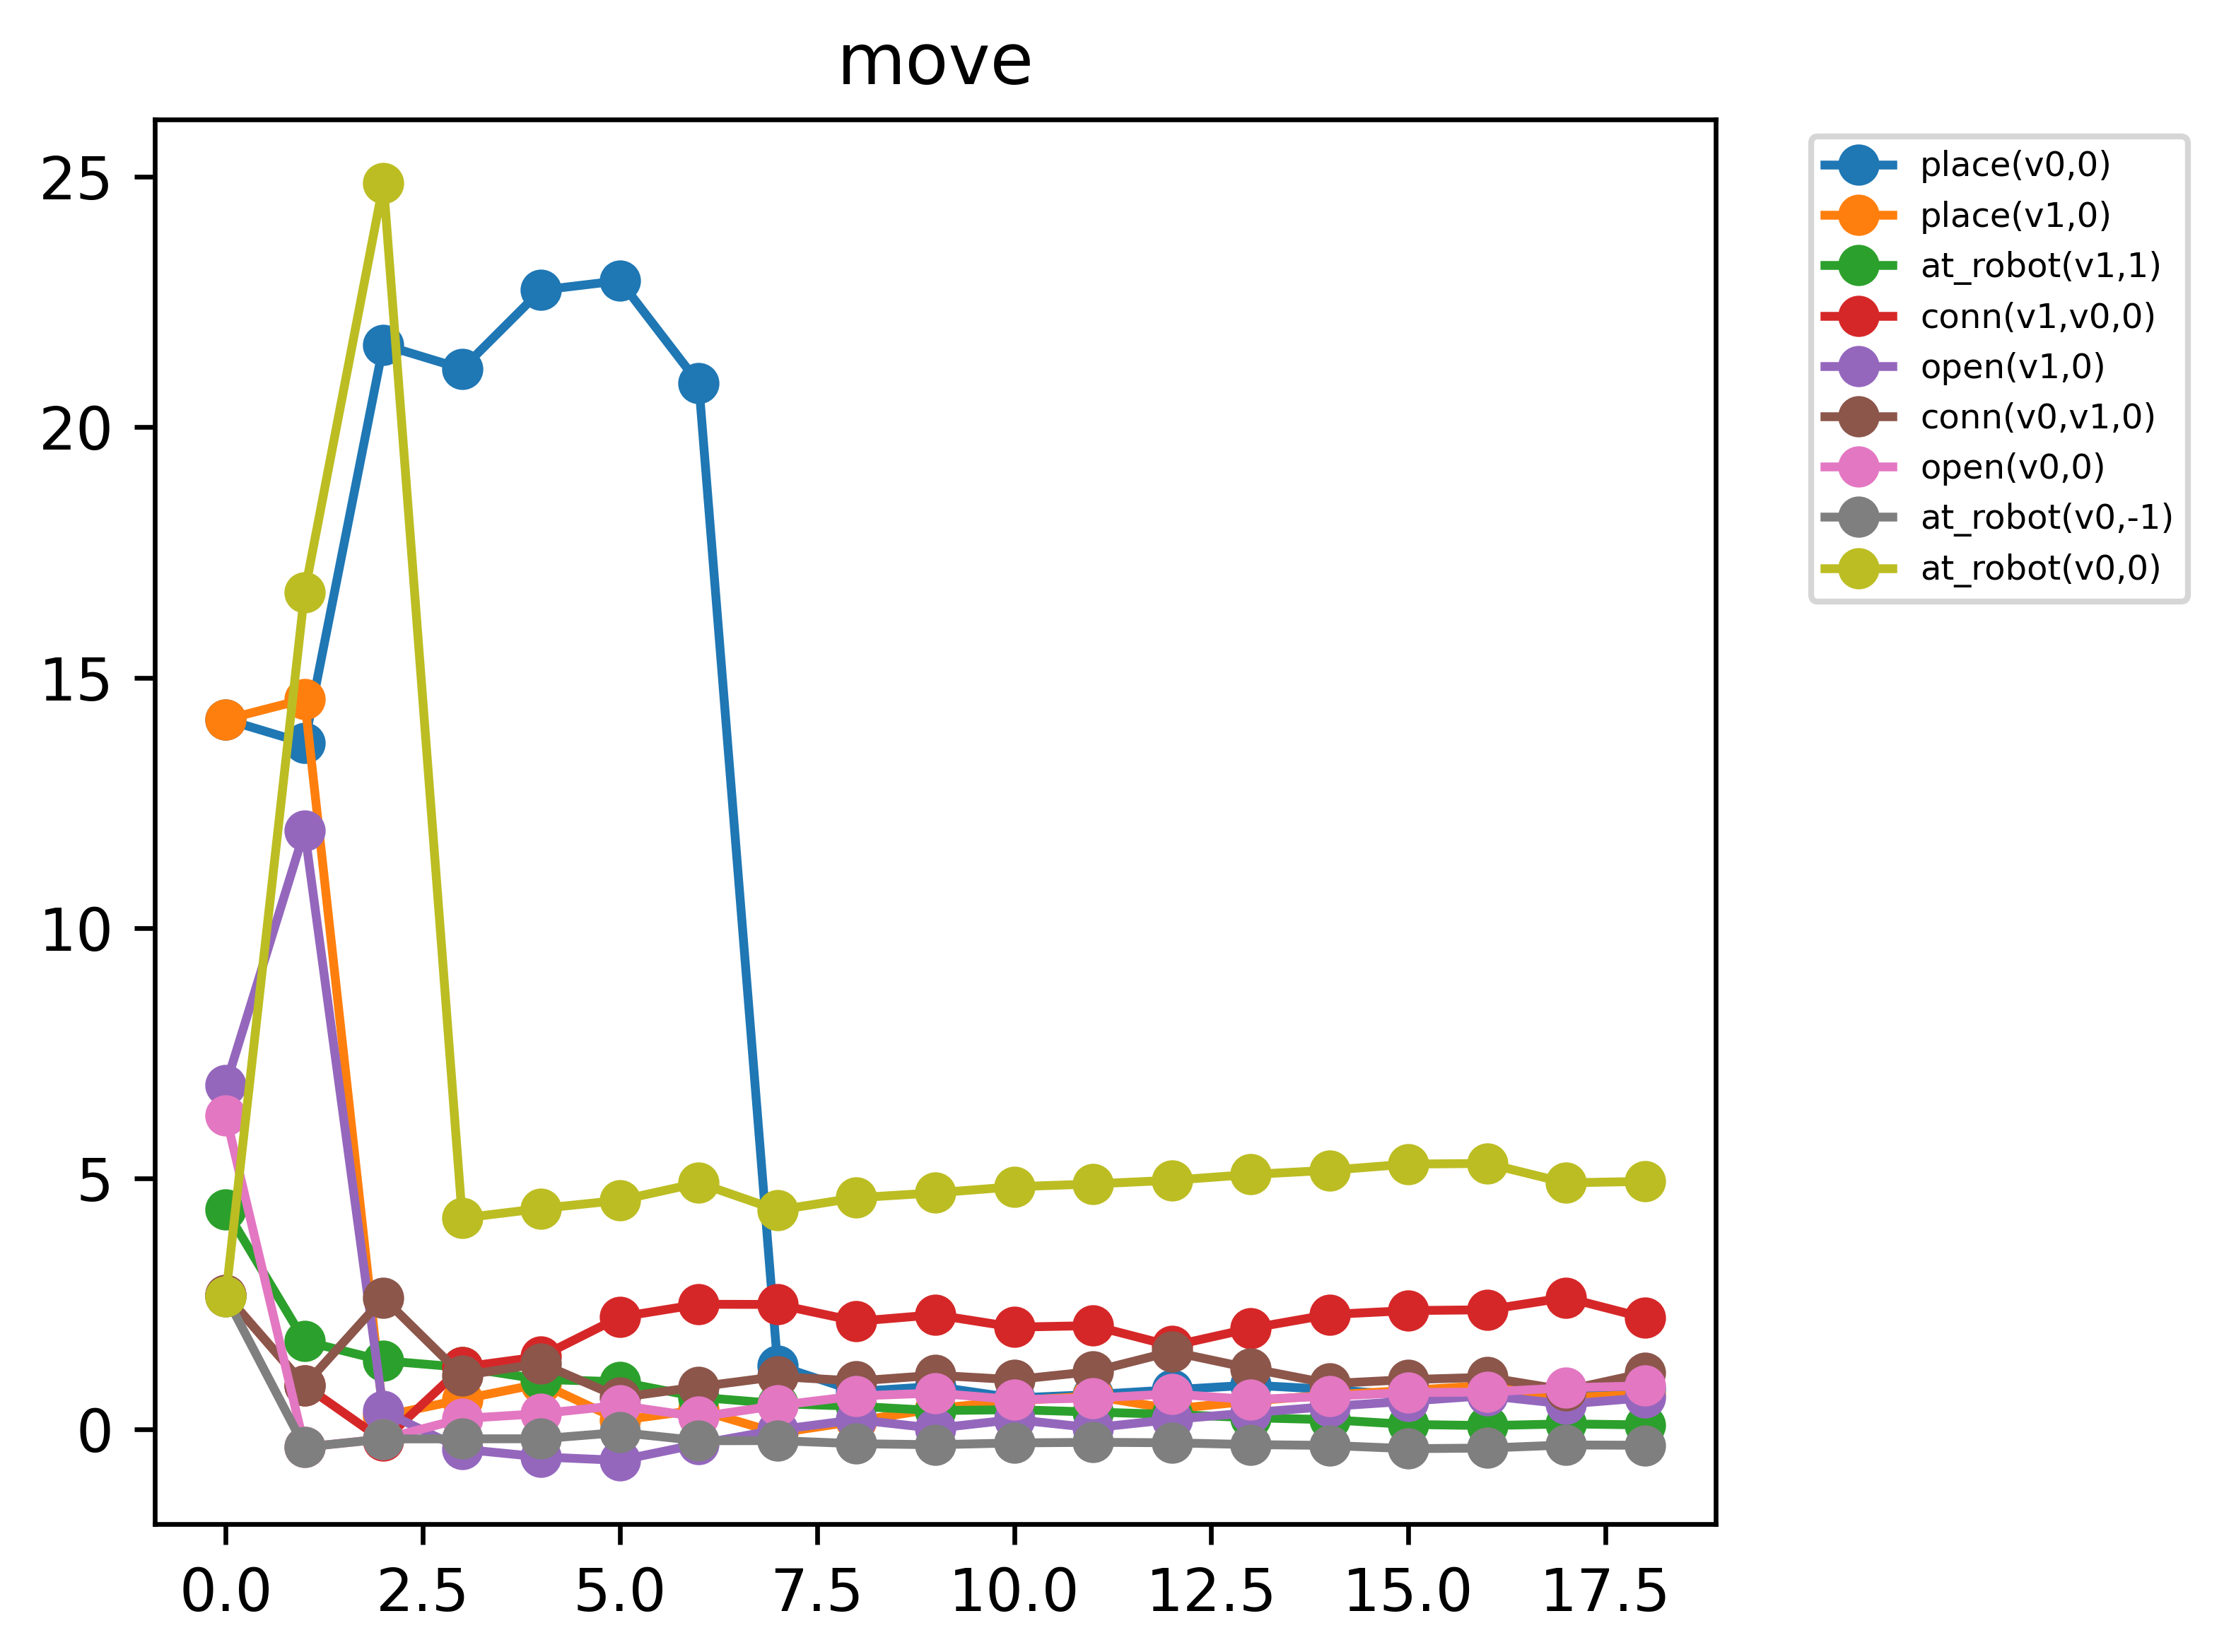
\includegraphics[width=1\textwidth]{images/tests/movegraph_rand_70}
 \caption{Move action MLN, .3 rand noise {fig:mv}}

 \end{minipage}
 \hfill
 \begin{minipage}[b]{0.49\linewidth}

 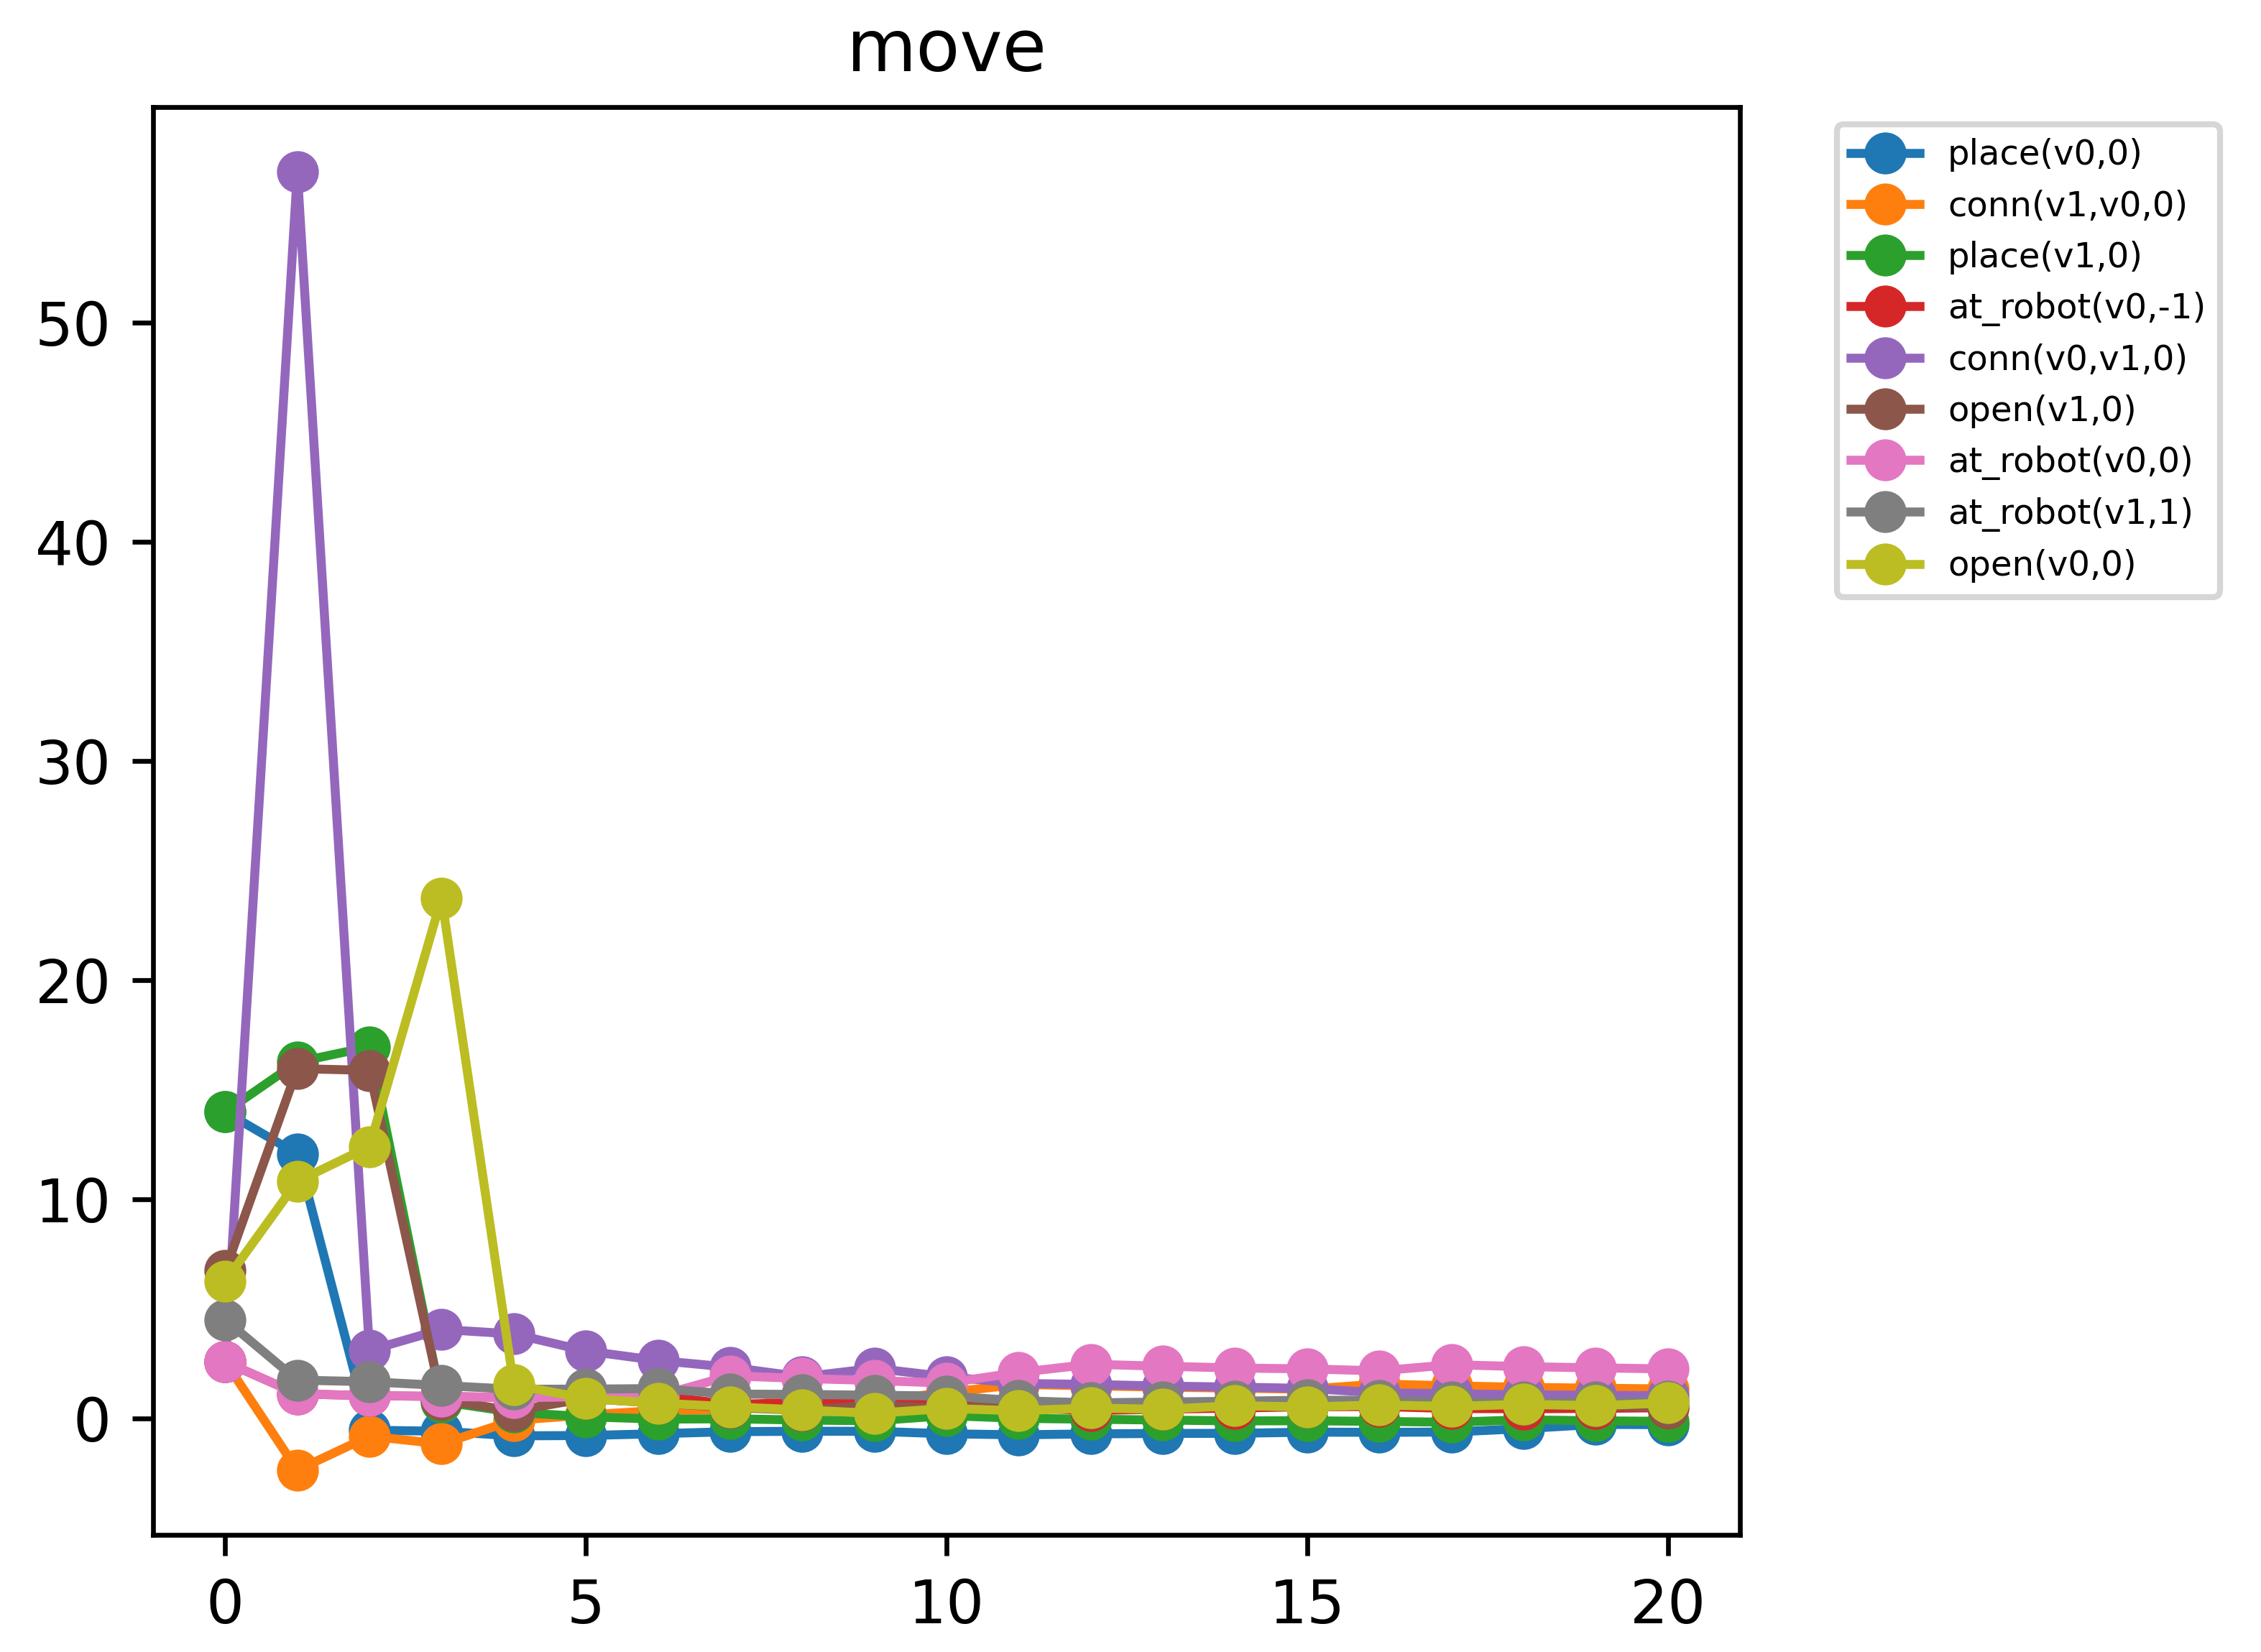
\includegraphics[width=1\textwidth]{images/tests/movegraph_rand_30}
 \caption{Move action MLN, .7 rand noise on){fig:mv_100_cum}}

 \end{minipage}
\end{figure}

\begin{figure}[h]
 \centering
 \begin{minipage}[b]{0.49\linewidth}
 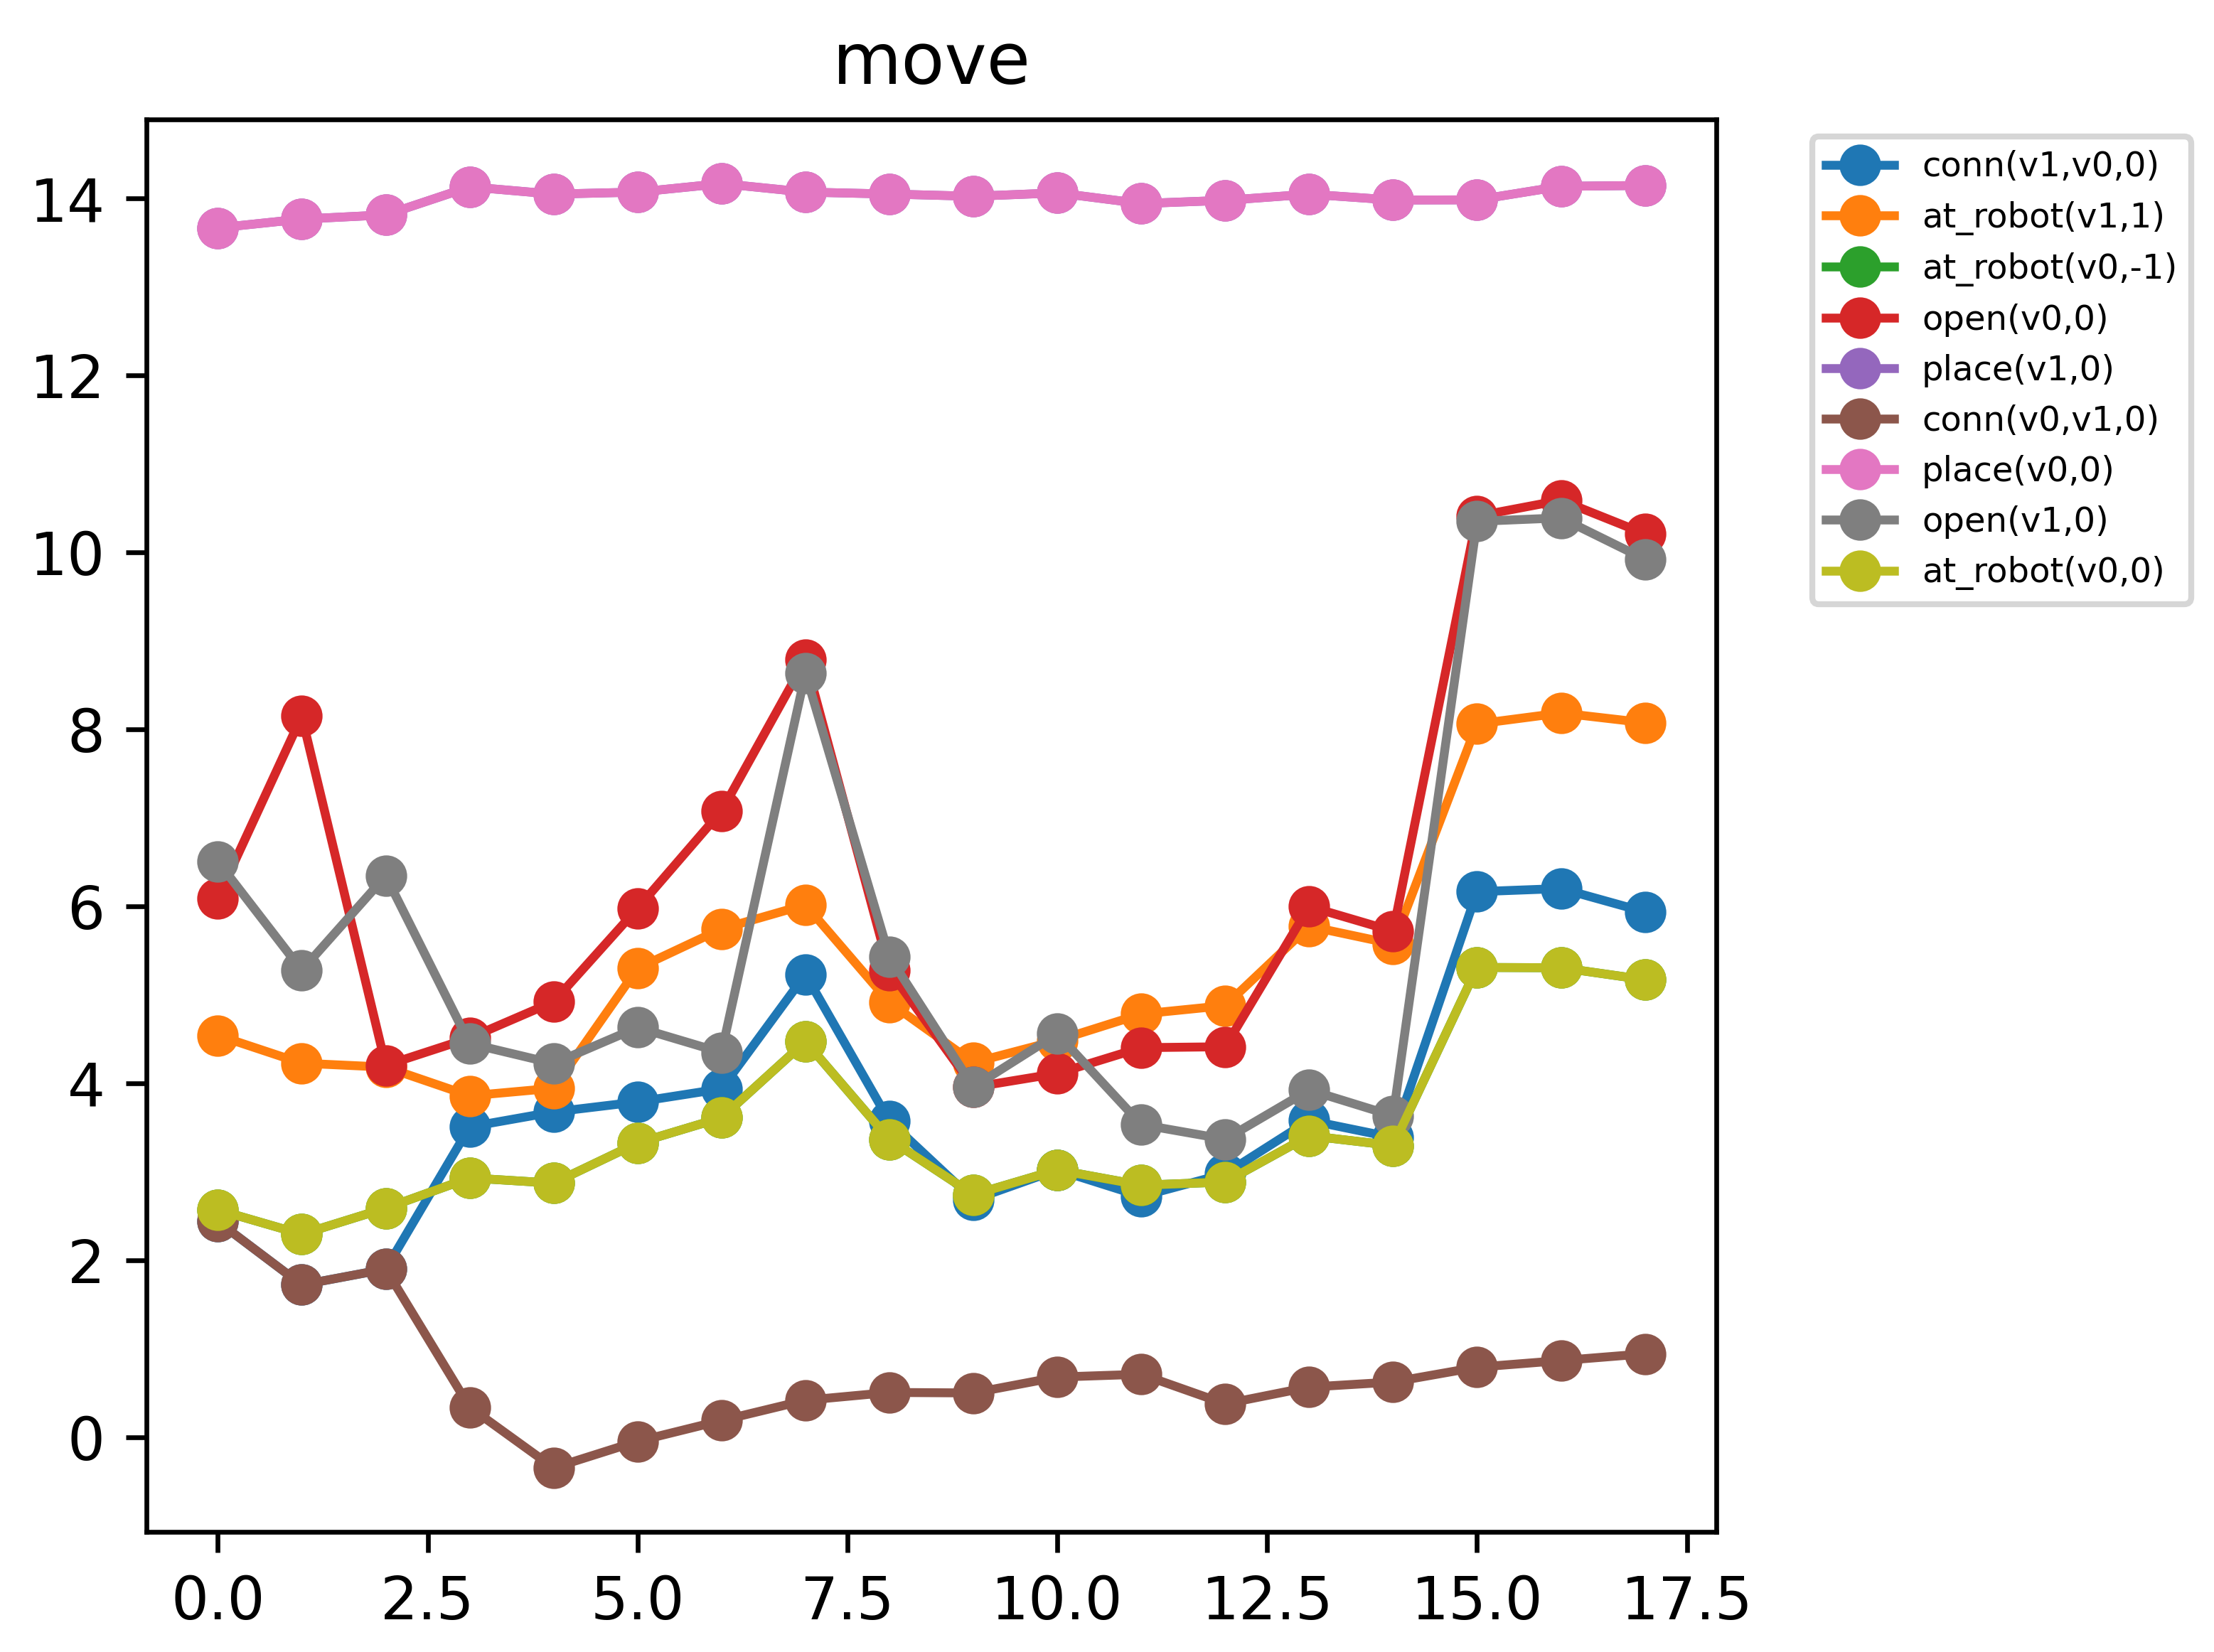
\includegraphics[width=1\textwidth]{images/tests/movegraph_sys_70}
 \caption{Move action MLN, .3 sys noise on conn(v0,v1,0) {fig:mv_100}}

 \end{minipage}
 \hfill
 \begin{minipage}[b]{0.49\linewidth}

 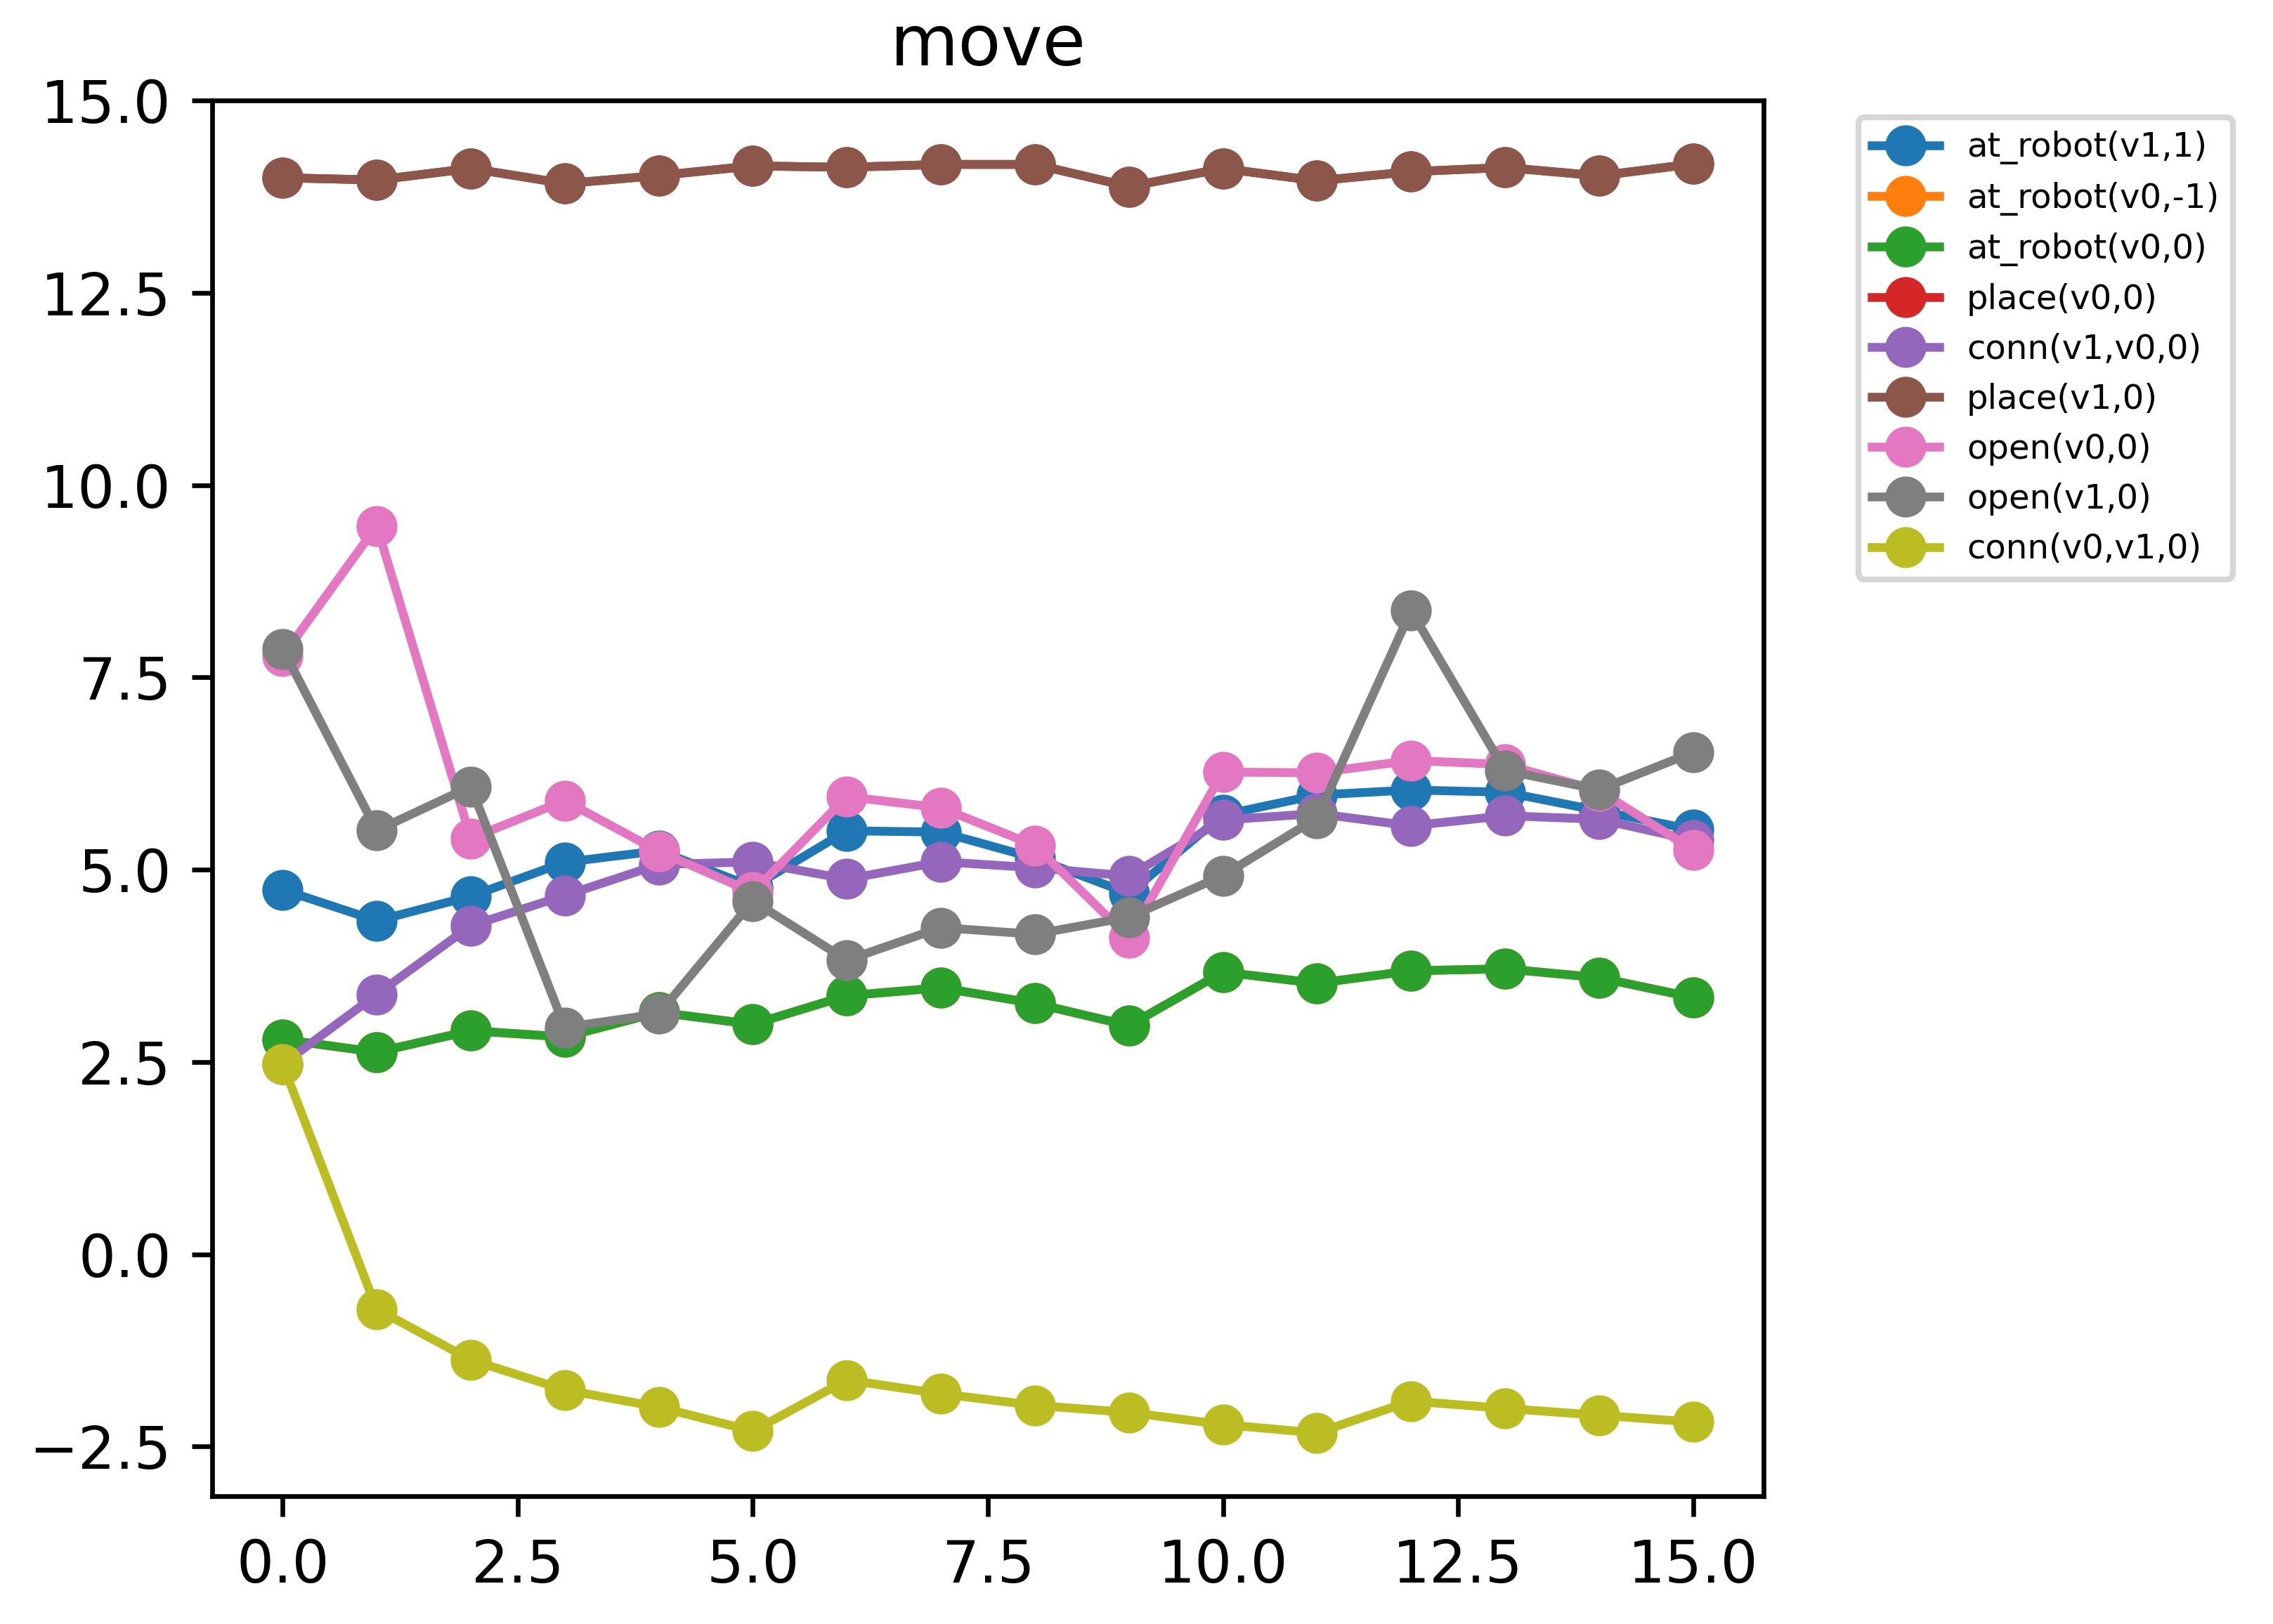
\includegraphics[width=1\textwidth]{images/tests/movegraph_sys_30}
 \caption{Move action MLN, .7 sys noise on conn(v0,v1,0){fig:mv_100_cum}}

 \end{minipage}
\end{figure}
\newpage
As we can observe from the above data, Although weights will reduce with noise. If we include predicates unrelated to the model, these will reduce much faster than noisy weights, this would allow us to recreate an action model from the network. \newline\newline
The greatest issue with this approach is not the viability of the technique but the efficiency of it. To train 25 database containing multiple actions, it takes around 30s to 1min, a multicore approach was not implemented in the pracmln package used for training, and a multitude of optimizations and fixes were done in order to speed up training and errors (optimizing data structures, operations over arrays, improperly handled exceptions, a fixed package has been uploaded to the project). A partial rewrite of the package for training MLN's online is required in order to use this technique on any moderately serious domains (>20 predicates). Optimizations include multithreading the training process, optimizing operation over grounded predicates and weights.\newline\newline
The results in the figures provided were created by training MLN's on pruned weights as forgoing this step made training impossible. Training speed reduces significantly when the number of weights are doubled or tripled which is a common occurrence in a normal domain.
\chapter{Conclusion}


\bibliographystyle{plain}
\bibliography{bibliography}

\end{document}


